\pdfoutput=1

%\documentclass[preprint,10pt]{elsarticle}
\documentclass[preprint,10pt]{article}
%\documentclass[review]{siamart0216}
%\documentclass{siamart0216}

\usepackage{fullpage}
\usepackage[colorlinks=true]{hyperref}

\usepackage{amsmath,amssymb,amsfonts,amsthm}
\theoremstyle{definition}
\newtheorem{definition}{Definition}
\theoremstyle{lemma}
\newtheorem{lemma}{Lemma}
\newtheorem*{remark}{Remark}
\theoremstyle{theorem}
\newtheorem{theorem}{Theorem}
\theoremstyle{assumption}
\newtheorem{assumption}{Assumption}

\usepackage[titletoc,toc,title]{appendix}

\usepackage{array} 
\usepackage{mathtools}
\usepackage{pdfpages}
\usepackage{bm}
\usepackage{bbm}

\usepackage{tikz}
\usepackage[normalem]{ulem}
\usepackage{hhline}

\usepackage{graphicx}
\usepackage{subfig}
\usepackage{color}

%% ====================================== graphics

\usepackage{pgfplots}
\usepackage{pgfplotstable}
\definecolor{markercolor}{RGB}{124.9, 255, 160.65}
\pgfplotsset{
compat=1.3,
width=10cm,
tick label style={font=\small},
label style={font=\small},
legend style={font=\small}
}

\usetikzlibrary{calc}
\usetikzlibrary{intersections} 

%%% START MACRO FOR ANNOTATION OF TRIANGLE WITH SLOPE %%%.
\newcommand{\logLogSlopeTriangle}[5]
{
    % #1. Relative offset in x direction.
    % #2. Width in x direction, so xA-xB.
    % #3. Relative offset in y direction.
    % #4. Slope d(y)/d(log10(x)).
    % #5. Plot options.

    \pgfplotsextra
    {
        \pgfkeysgetvalue{/pgfplots/xmin}{\xmin}
        \pgfkeysgetvalue{/pgfplots/xmax}{\xmax}
        \pgfkeysgetvalue{/pgfplots/ymin}{\ymin}
        \pgfkeysgetvalue{/pgfplots/ymax}{\ymax}

        % Calculate auxilliary quantities, in relative sense.
        \pgfmathsetmacro{\xArel}{#1}
        \pgfmathsetmacro{\yArel}{#3}
        \pgfmathsetmacro{\xBrel}{#1-#2}
        \pgfmathsetmacro{\yBrel}{\yArel}
        \pgfmathsetmacro{\xCrel}{\xArel}

        \pgfmathsetmacro{\lnxB}{\xmin*(1-(#1-#2))+\xmax*(#1-#2)} % in [xmin,xmax].
        \pgfmathsetmacro{\lnxA}{\xmin*(1-#1)+\xmax*#1} % in [xmin,xmax].
        \pgfmathsetmacro{\lnyA}{\ymin*(1-#3)+\ymax*#3} % in [ymin,ymax].
        \pgfmathsetmacro{\lnyC}{\lnyA+#4*(\lnxA-\lnxB)}
        \pgfmathsetmacro{\yCrel}{\lnyC-\ymin)/(\ymax-\ymin)} % THE IMPROVED EXPRESSION WITHOUT 'DIMENSION TOO LARGE' ERROR.

        % Define coordinates for \draw. MIND THE 'rel axis cs' as opposed to the 'axis cs'.
        \coordinate (A) at (rel axis cs:\xArel,\yArel);
        \coordinate (B) at (rel axis cs:\xBrel,\yBrel);
        \coordinate (C) at (rel axis cs:\xCrel,\yCrel);

        % Draw slope triangle.
        \draw[#5]   (A)-- node[pos=0.5,anchor=north] {}
                    (B)-- 
                    (C)-- node[pos=0.5,anchor=west] {#4}
                    cycle;
    }
}
%%% END MACRO FOR ANNOTATION OF TRIANGLE WITH SLOPE %%%.

\newcommand{\logLogSlopeTriangleNeg}[5]
{
    % #1. Relative offset in x direction.
    % #2. Width in x direction, so xA-xB.
    % #3. Relative offset in y direction.
    % #4. Slope d(y)/d(log10(x)).
    % #5. Plot options.

    \pgfplotsextra
    {
        \pgfkeysgetvalue{/pgfplots/xmin}{\xmin}
        \pgfkeysgetvalue{/pgfplots/xmax}{\xmax}
        \pgfkeysgetvalue{/pgfplots/ymin}{\ymin}
        \pgfkeysgetvalue{/pgfplots/ymax}{\ymax}

        % Calculate auxilliary quantities, in relative sense.
        \pgfmathsetmacro{\xArel}{#1}
        \pgfmathsetmacro{\yArel}{#3}
        \pgfmathsetmacro{\xBrel}{#1-#2}
        \pgfmathsetmacro{\yBrel}{\yArel}
        \pgfmathsetmacro{\xCrel}{\xArel}

        \pgfmathsetmacro{\lnxB}{\xmin*(1-(#1-#2))+\xmax*(#1-#2)} % in [xmin,xmax].
        \pgfmathsetmacro{\lnxA}{\xmin*(1-#1)+\xmax*#1} % in [xmin,xmax].
        \pgfmathsetmacro{\lnyA}{\ymin*(1-#3)+\ymax*#3} % in [ymin,ymax].
        \pgfmathsetmacro{\lnyC}{\lnyA+#4*(\lnxA-\lnxB)}
        \pgfmathsetmacro{\yCrel}{\lnyC-\ymin)/(\ymax-\ymin)} % THE IMPROVED EXPRESSION WITHOUT 'DIMENSION TOO LARGE' ERROR.

        % Define coordinates for \draw. MIND THE 'rel axis cs' as opposed to the 'axis cs'.
        \coordinate (A) at (rel axis cs:\xArel,\yArel);
        \coordinate (B) at (rel axis cs:\xBrel,\yBrel);
        \coordinate (C) at (rel axis cs:\xCrel,\yCrel);

        % Draw slope triangle.
        \draw[#5]   (A)-- node[pos=.5,anchor=south] {}
                    (B)-- 
                    (C)-- node[pos=0.5,anchor=west] {#4}
                    cycle;
    }
}
%%% END MACRO FOR ANNOTATION OF TRIANGLE WITH SLOPE %%%.

%%% START MACRO FOR ANNOTATION OF TRIANGLE WITH SLOPE %%%.
\newcommand{\logLogSlopeTriangleFlipNeg}[5]
{
    % #1. Relative offset in x direction.
    % #2. Width in x direction, so xA-xB.
    % #3. Relative offset in y direction.
    % #4. Slope d(y)/d(log10(x)).
    % #5. Plot options.

    \pgfplotsextra
    {
        \pgfkeysgetvalue{/pgfplots/xmin}{\xmin}
        \pgfkeysgetvalue{/pgfplots/xmax}{\xmax}
        \pgfkeysgetvalue{/pgfplots/ymin}{\ymin}
        \pgfkeysgetvalue{/pgfplots/ymax}{\ymax}

        % Calculate auxilliary quantities, in relative sense.
        %\pgfmathsetmacro{\xArel}{#1}
        %\pgfmathsetmacro{\yArel}{#3}
        \pgfmathsetmacro{\xBrel}{#1-#2}
        \pgfmathsetmacro{\yBrel}{#3}
        \pgfmathsetmacro{\xCrel}{#1}

        \pgfmathsetmacro{\lnxB}{\xmin*(1-(#1-#2))+\xmax*(#1-#2)} % in [xmin,xmax].
        \pgfmathsetmacro{\lnxA}{\xmin*(1-#1)+\xmax*#1} % in [xmin,xmax].
        \pgfmathsetmacro{\lnyA}{\ymin*(1-#3)+\ymax*#3} % in [ymin,ymax].
        \pgfmathsetmacro{\lnyC}{\lnyA+#4*(\lnxA-\lnxB)}
        \pgfmathsetmacro{\yCrel}{\lnyC-\ymin)/(\ymax-\ymin)} % THE IMPROVED EXPRESSION WITHOUT 'DIMENSION TOO LARGE' ERROR.

	\pgfmathsetmacro{\xArel}{\xBrel}
        \pgfmathsetmacro{\yArel}{\yCrel}

        % Define coordinates for \draw. MIND THE 'rel axis cs' as opposed to the 'axis cs'.
        \coordinate (A) at (rel axis cs:\xArel,\yArel);
        \coordinate (B) at (rel axis cs:\xBrel,\yBrel);
        \coordinate (C) at (rel axis cs:\xCrel,\yCrel);

        % Draw slope triangle.
        \draw[#5]   (A)-- node[pos=0.5,anchor=east] {#4}
                    (B)-- 
                    (C)-- node[pos=0.5,anchor=north] {1}
                    cycle;
    }
}
%%% END MACRO FOR ANNOTATION OF TRIANGLE WITH SLOPE %%%.


%%% START MACRO FOR ANNOTATION OF TRIANGLE WITH SLOPE %%%.
\newcommand{\logLogSlopeTriangleFlip}[5]
{
    % #1. Relative offset in x direction.
    % #2. Width in x direction, so xA-xB.
    % #3. Relative offset in y direction.
    % #4. Slope d(y)/d(log10(x)).
    % #5. Plot options.

    \pgfplotsextra
    {
        \pgfkeysgetvalue{/pgfplots/xmin}{\xmin}
        \pgfkeysgetvalue{/pgfplots/xmax}{\xmax}
        \pgfkeysgetvalue{/pgfplots/ymin}{\ymin}
        \pgfkeysgetvalue{/pgfplots/ymax}{\ymax}

        % Calculate auxilliary quantities, in relative sense.
        %\pgfmathsetmacro{\xArel}{#1}
        %\pgfmathsetmacro{\yArel}{#3}
        \pgfmathsetmacro{\xBrel}{#1-#2}
        \pgfmathsetmacro{\yBrel}{#3}
        \pgfmathsetmacro{\xCrel}{#1}

        \pgfmathsetmacro{\lnxB}{\xmin*(1-(#1-#2))+\xmax*(#1-#2)} % in [xmin,xmax].
        \pgfmathsetmacro{\lnxA}{\xmin*(1-#1)+\xmax*#1} % in [xmin,xmax].
        \pgfmathsetmacro{\lnyA}{\ymin*(1-#3)+\ymax*#3} % in [ymin,ymax].
        \pgfmathsetmacro{\lnyC}{\lnyA+#4*(\lnxA-\lnxB)}
        \pgfmathsetmacro{\yCrel}{\lnyC-\ymin)/(\ymax-\ymin)} % THE IMPROVED EXPRESSION WITHOUT 'DIMENSION TOO LARGE' ERROR.

	\pgfmathsetmacro{\xArel}{\xBrel}
        \pgfmathsetmacro{\yArel}{\yCrel}

        % Define coordinates for \draw. MIND THE 'rel axis cs' as opposed to the 'axis cs'.
        \coordinate (A) at (rel axis cs:\xArel,\yArel);
        \coordinate (B) at (rel axis cs:\xBrel,\yBrel);
        \coordinate (C) at (rel axis cs:\xCrel,\yCrel);

        % Draw slope triangle.
        \draw[#5]   (A)-- node[pos=0.5,anchor=east] {#4}
                    (B)-- 
                    (C)-- node[pos=0.5,anchor=south] {}
                    cycle;
    }
}
%%% END MACRO FOR ANNOTATION OF TRIANGLE WITH SLOPE %%%.


\renewcommand{\topfraction}{0.85}
\renewcommand{\textfraction}{0.1}
\renewcommand{\floatpagefraction}{0.75}


\newcommand{\bbm}[1]{\mathbbm{#1}}
\newcommand{\bs}[1]{\boldsymbol{#1}}
\newcommand{\equaldef}{\stackrel{\mathrm{def}}{=}}


\newcommand{\mb}[1]{\mathbf{#1}}
\newcommand{\mbb}[1]{\mathbb{#1}}
\newcommand{\mc}[1]{\mathcal{#1}}

\renewcommand{\hat}{\widehat}
\renewcommand{\tilde}{\widetilde}
\newcommand{\td}[2]{\frac{{\rm d}#1}{{\rm d}{\rm #2}}}
\newcommand{\pd}[2]{\frac{\partial#1}{\partial#2}}
\newcommand{\pdn}[3]{\frac{\partial^{#3}#1}{\partial#2^{#3}}}
\newcommand{\snor}[1]{\left| #1 \right|}
\newcommand{\nor}[1]{\left\| #1 \right\|}
\newcommand{\LRp}[1]{\left( #1 \right)}
\newcommand{\LRs}[1]{\left[ #1 \right]}
\newcommand{\LRa}[1]{\left\langle #1 \right\rangle}
\newcommand{\LRb}[1]{\left| #1 \right|}
\newcommand{\LRc}[1]{\left\{ #1 \right\}}
\newcommand{\LRceil}[1]{\left\lceil #1 \right\rceil}
\newcommand{\LRl}[1]{\left. \LRp{#1} \right|}
\newcommand{\jump}[1] {\ensuremath{\llbracket#1\rrbracket}}
\newcommand{\avg}[1] {\ensuremath{\LRc{\!\{#1\}\!}}}
\newcommand{\Grad} {\ensuremath{\nabla}}
\newcommand{\note}[1]{{\color{blue}{#1}}}
\renewcommand{\d}{\partial}


\newcommand{\LK}{L^2\LRp{D^k}}
\newcommand{\LdK}{L^2\LRp{\partial D^k}}
\newcommand{\Dhat}{\widehat{D}}
\newcommand{\Lhat}{L^2\LRp{\Dhat}}


\newcommand*\diff[1]{\mathop{}\!{\mathrm{d}#1}} % d in integrand

\date{}
\author{Jesse Chan, Lucas Wilcox}
\title{Discretely entropy stable weight-adjusted discontinuous Galerkin methods: curvilinear meshes and GPU acceleration}
\graphicspath{{./figs/}}


\begin{document}

\maketitle

\begin{abstract}
We construct entropy conservative and entropy stable high order discontinuous Galerkin (DG) discretizations for time-dependent nonlinear hyperbolic conservation laws on curvilinear meshes by extending the methodology of \cite{chan2017discretely}.  The resulting schemes preserve a semi-discrete form of the continuous entropy inequality and guaranteeing that the semi-discrete solution is stable in time.  The proof of stability requires the satisfaction of a discrete geometric conservation law, which we enforce through a modification of \cite{kopriva2006metric}.  We also describe how to construct entropy conservative and entropy stable DG schemes using low-storage weight-adjusted approximations to high order curvilinear mass matrices \cite{chan2016weight1, chan2016weight2} based on a high order accurate weight-adjusted projection operator.  We present numerical experiments which verify theoretical results for the compressible Euler equations in two and three dimensions.
%Things to include: entropy conservation and stability on curvilinear meshes, choosing geometric terms to ensure constant state preservation, high order accuracy.  Computational considerations for curvilinear meshes.  
\end{abstract}

\tableofcontents

\section{Introduction}

Introducing WADG \cite{chan2016weight1,chan2016weight2}.  

Matrix WADG: GPU efficiency of WADG vs storing weighted inverses \cite{chan2017weight}.  

\section{Systems of nonlinear conservation laws}

This work addresses is high order schemes for the following system of $n$ nonlinear conservation laws in $d$ dimensions 
\begin{equation}
\pd{\bm{u}}{t} + \sum_{j=1}^d\pd{\bm{f}_j(\bm{u})}{x_j}  = 0, \qquad \bm{u} \in \mathbb{R}^n, \qquad \bm{f}_j : \mathbb{R}^n\rightarrow \mathbb{R}^n,
\label{eq:nonlineqs}
\end{equation}
where $\bm{u}(\bm{x},t)$ denote the \emph{conservative variables} for this system.  We will specify boundary conditions in a later section.  

We are interested in nonlinear conservation laws for which an entropy function $U(\bm{u})$ exists, where $U(\bm{u})$ is convex with respect to the conservative variables $\bm{u}$.  If this function exists, then it is possible to define \emph{entropy variables} $\bm{v}(\bm{u}) = \pd{U}{\bm{u}}$.  These functions symmetrize the system of nonlinear conservation laws (\ref{eq:nonlineqs}) \cite{hughes1986new}.  

It can be shown (see, for example, \cite{mock1980systems}) that symmetrization is equivalent to the existence of an entropy flux function $F(\bm{u})$ and entropy potential $\psi$ such that
\[
\bm{v}^T \pd{\bm{f}_j}{\bm{u}} = \pd{F_j(\bm{u})}{\bm{u}}^T, \qquad \psi_j(\bm{v}) = \bm{v}^T\bm{f}_j(\bm{u}(\bm{v})) - F_j(\bm{u}(\bm{v})), \qquad \psi_j'(\bm{v}) = \bm{f}_j(\bm{u}(\bm{v})).
\]
Smooth solutions of (\ref{eq:nonlineqs}) can be shown to satisfy a conservation of entropy by multiplying (\ref{eq:nonlineqs}) by $\bm{v}(\bm{u})$. Using the definition of the entropy variables, entropy flux, and the chain rule yields 
\begin{equation}
\bm{v}^T\pd{\bm{f}_j(\bm{u})}{x_j} = \pd{U(\bm{u})}{\bm{u}}^T\pd{\bm{f}_j(\bm{u})}{\bm{u}}\pd{\bm{u}}{x_j} = \pd{F_j(\bm{u})}{x_j},
\label{eq:chainrule}
\end{equation}
and that 
\begin{equation*}
\pd{U(\bm{u})}{t} + \sum_{j=1}^d \pd{F_j(\bm{u})}{x_j} = 0.
%\label{eq:entropyeqstrong}
\end{equation*}
Let $\Omega\mathbb{R}^d$ now be a closed domain with boundary $\partial \Omega$.  Integrating over $\Omega$ an using Gauss' theorem on the spatial derivative yields
\begin{equation}
\int_{\Omega}\pd{U(\bm{u})}{t}\diff{x} + \int_{\partial \Omega} \sum_{j=1}^d \LRp{\bm{v}(\bm{u})^T\bm{f}_j(\bm{u}) - \psi_j\LRp{\bm{v}(\bm{u})}}n_j \diff{x} = 0,
\label{eq:entropyeq}
\end{equation}
where $\bm{n} = \LRp{n_1,\ldots,n_d}^T$ denotes the unit outward normal vector on $\partial \Omega$.  

General solutions (including non-smooth solutions such as shocks) satisfy an entropy \emph{inequality}
\begin{equation}
\int_{\Omega}\pd{U(\bm{u})}{t}\diff{x} + \int_{\partial \Omega} \sum_{j=1}^d \LRp{\bm{v}(\bm{u})^T\bm{f}_j(\bm{u}) - \psi_j\LRp{\bm{v}(\bm{u})}}n_j \diff{x} \leq 0,
\label{eq:entropyineq}
\end{equation}
which results from considering solutions of an appropriate viscous form of the equations (\ref{eq:nonlineqs}) and taking the limit as viscosity vanishes.  In this work, schemes which satisfy a discrete form of (\ref{eq:entropyineq}) will be constructed by first enforcing a discrete version of entropy conservation (\ref{eq:entropyeq}), then adding an appropriate numerical dissipation which will enforce the entropy inequality (\ref{eq:entropyineq}).  


\subsection{Standard DG formulations for nonlinear conservation laws}

We begin by reviewing the construction of standard high order DG formulations for (\ref{eq:nonlineqs}).  

\subsubsection{Mathematical notation}

Let the domain $\Omega \subset \mathbb{R}^d$ be decomposed into elements (subdomains) $D^k$, and let $\hat{D}$ denote a $d$-dimensional reference element with boundary $\partial \hat{D}$.  Let $\hat{\bm{x}} = \LRc{\hat{x}_1,\ldots,\hat{x}_d}$ denote coordinates on $\hat{D}$, and let $\hat{n}_i$ denote and the $i$th component of the unit normal vector on $\partial \hat{D}$.  We assume that $\hat{n}_i$ is constant; i.e., that the faces of the reference element are planar (this assumption holds for all commonly used reference elements \cite{chan2015gpu}).  

We will assume that each physical element $D^k$ is the image of $\hat{D}$ under some smoothly differentiable mapping $\bm{\Phi}_k(\hat{\bm{x}})$ such that
\[
\bm{x} = \bm{\Phi}_k(\hat{\bm{x}}), \qquad \bm{x}\in D^k.
\]
This also implies that integrals over physical elements can be mapped back to the reference element as follows
\[
\int_{D^k} u \diff{\bm{x}} = \int_{\hat{D}} u J^k\diff{\hat{\bm{x}}}, 
\]
where $J^k$ denotes the determinant of the Jacobian of $\bm{\Phi}_k$.  Integrals over physical faces of $D^k$ can similarly be mapped back to reference faces.


We define an approximation space using degree $N$ polynomials on the reference element.  For example, on a $d$-dimensional reference simplex, the natural polynomial space are total degree $N$ polynomials 
\[
P^N\LRp{\widehat{D}} = \LRc{\hat{x}_1^{i_1}\ldots\hat{x}_d^{i_d}, \quad \hat{\bm{x}} \in \widehat{D}, \quad 0\leq \sum_{k=1}^d i_k \leq N}.
\]
Other element types possess different natural polynomial spaces \cite{chan2015gpu}, but typically contain the space of total degree $N$ polynomials.  This work is directly applicable to other elements and spaces as well.  We denote the dimension of the approximation space $P^N$ as $N_p = {\rm dim}\LRp{P^N\LRp{\widehat{D}}}$.  We also define trace spaces for each face of the reference element.  Let $\hat{f}$ be a face of the reference element $\hat{D}$.  The trace space over $\hat{f}$ is defined as the space of traces of functions in $P^N\LRp{\hat{D}}$
\[
P^N_f \LRp{\hat{f}} = \LRc{ \left.u\right|_{\hat{f}}, \quad u \in P^N\LRp{\hat{D}}}, \qquad \hat{f}\in \partial\hat{D}.
\]
We denote the dimension of the trace space as ${\rm dim}P^N_f\LRp{\hat{f}} = N^f_p$.

Finally, we define the $L^2$ norm and inner products over the reference element $\hat{D}$ and the surface of the reference element $\partial \hat{D}$
\[
\LRp{\bm{u},\bm{v}}_{\hat{D}} = \int_{\hat{D}} \bm{u}\cdot\bm{v}\diff{\bm{x}} =  \int_{\widehat{D}} \bm{u}\cdot\bm{v} J^k \diff{\widehat{x}}, \qquad \nor{\bm{u}}^2_{\hat{D}} = (\bm{u},\bm{u})_{\hat{D}}, \qquad \LRa{\bm{u},\bm{v}}_{\partial \hat{D}} = \int_{\partial \hat{D}} \bm{u} \cdot \bm{v} \diff{\bm{x}},
\]
Finally, we introduce the continuous $L^2$ projection operator $\Pi_N$ and lifting operator $L$.  For $u \in L^2\LRp{\widehat{D}}$, the $L^2$ projection $\Pi_N u$ is defined through
\begin{equation}
\int_{\widehat{D}} \Pi_N u v \diff{\hat{\bm{x}}} = \int_{\widehat{D}} u v \diff{\hat{\bm{x}}}, \qquad \forall v\in P^N\LRp{\hat{D}}.
\label{eq:l2proj}
\end{equation}
Likewise, for a boundary function $u \in L^2\LRp{\partial \hat{D}}$, the lifting operator $L$ \cite{hesthaven2007nodal, di2011mathematical} is defined through 
\begin{equation}
\LRp{L u,v}_{\hat{D}} = \LRa{u,v}_{\partial \hat{D}}, \qquad \forall v \in P^N\LRp{\hat{D}}.
\label{eq:lift}
\end{equation}


\subsubsection{Discontinuous Galerkin formulations and the $L^2$ projection}

Discontinuous Galerkin methods have been very widely applied to systems of nonlinear conservation laws (\ref{eq:nonlineqs}) \cite{cockburn1989tvb, cockburn1998runge, cockburn2001devising, karniadakis2013spectral}.  The development of new discontinuous Galerkin methods for nonlinear conservation laws have focused heavily on the choice of numerical flux \cite{qiu2006numerical} or the development of  slope limiters \cite{krivodonova2007limiters, zhang2012maximum, dumbser2014posteriori} and artificial viscosity strategies \cite{persson2006sub, barter2010shock, klockner2011viscous}.  However, the treatment of the underlying volume discretization remains relatively unchanged between each of these approaches.  

Ignoring terms involving filters, limiters, or artificial viscosity, a semi-discrete ``weak'' DG formulation  for (\ref{eq:nonlineqs}) can be given locally over an element $D^k$: find $\bm{u}\in \LRp{P^N\LRp{D^k}}^n$ such that
\begin{align}
\int_{D^k} \LRp{\pd{\bm{u}}{t}\cdot \bm{v} - \sum_{j=1}^d\bm{f}_j(\bm{u}) \cdot \pd{\bm{v}}{x_i}} \diff{\bm{x}} 
+ \sum_{j=1}^d \int_{\partial D^k} \LRp{\bm{f}^*_j\LRp{\bm{u}^+,\bm{u}} }\cdot \bm{v} n_j  \diff{\bm{x}} = 0, \qquad \forall \bm{v}\in \LRp{P^N\LRp{D^k}}^n,
\label{eq:weakdg}
\end{align}
where the numerical flux $\bm{f}^*$ is a function of the solution $\bm{u}$ on both $D^k$ and neighboring elements.  

Unfortunately, solutions to (\ref{eq:weakdg}) do not (in general) obey a discrete version of the entropy inequality (\ref{eq:entropyineq}).  Since (\ref{eq:entropyineq}) is a generalized statement of energy stability, the lack of a discrete entropy inequality implies that the discrete solution can blow up in finite time.  The reason for this is due the fact that, in practice, the integrals in (\ref{eq:weakdg}) are not computed exactly and are instead approximated using polynomially exact quadratures.  This is compounded by the fact that the nonlinear flux  function $\bm{f}_j\LRp{\bm{u}}$ is often rational and impossible to integrate exactly using polynomial quadratures.  To account for the inexactness of quadrature, we rewrite (\ref{eq:weakdg}) in strong form using a discrete quadrature-based $L^2$ projection.  

For polynomial approximation spaces, $\pd{\bm{v}}{x_i}$ is polynomial.  Then, mapping (\ref{eq:weakdg}) back to the reference element $\hat{D}$ and using the $L^2$ projection and (\ref{eq:l2proj}), we have that
\[
\int_{D^k} \bm{f}_j(\bm{u}) \cdot \pd{\bm{v}}{x_i} \diff{\bm{x}} = \int_{\hat{D}} \Pi_N \bm{f}_j(\bm{u}) \cdot \pd{\bm{v}}{x_i} J^k\diff{\bm{x}}.
\]
Thus, integrating by parts (\ref{eq:weakdg}) recovers a ``strong'' DG formulation involving the projection operator
\begin{align}
&\int_{D^k} \LRp{\pd{\bm{u}}{t} - \sum_{j=1}^d \pd{\Pi_N \bm{f}_j(\bm{u})}{x_j}} \cdot \bm{v} \diff{\bm{x}} \nonumber\\
&+ \sum_{j=1}^d \int_{\partial D^k} \LRp{\bm{f}^*_j\LRp{\bm{u}^+,\bm{u}} - \Pi_N\bm{f}_j(\bm{u})}\cdot \bm{v} n_j  \diff{\bm{x}} = 0, \qquad \forall \bm{v}\in \LRp{P^N\LRp{D^k}}^n.  
\label{eq:strongdg}
\end{align}
From this, we see that our discrete scheme does not differentiation the nonlinear flux function $\bm{f}_j\LRp{\bm{u}}$ exactly, but instead differentiates the projection of $\Pi_N \bm{f}_j\LRp{\bm{u}}$ onto polynomials of degree $N$.  Because the $L^2$ projection operator is introduced, the chain rule no longer holds at the discrete level and step (\ref{eq:chainrule}) of the proof of entropy conservation is no longer valid.  Thus, ensuring discrete entropy stability will require a discrete formulation of the system of nonlinear conservation laws (\ref{eq:nonlineqs}) from which we can prove a discrete entropy inequality without relying on the chain rule.  

%We note that it is not strictly necessary to introduce the projection operator; however, constructing a ``strong'' DG formulation without a projection operator requires an analytical expression for derivatives of the nonlinear flux function $\bm{f}_j\LRp{\bm{u}}$, which can be complex or expensive to compute.  Moreover, because polynomial quadrature rules are typically used in practice to evaluate integrals, it is not possible to use integration by parts when the nonlinear flux function is rational due to errors in approximating integrals.  Introducing the $L^2$ projection operator resolves both issues, as the integrands involved in integration by parts are polynomials of degree $2N-1$, for which efficient quadratures exist. 

\section{Discretely entropy stable DG methods on curved meshes}

We will first show how to construct discretely entropy stable high order DG methods on curvilinear meshes, but will present this using a matrix formulation as opposed to a continuous formulation.  This is to ensure that the effects of discretization, nonlinear, and quadrature are accounted for in the proof of semi-discrete entropy stability.  We first introduce quadrature-based matrices, which we will then use to construct discretely entropy stable DG formulations.


\subsection{Basis and quadrature rules}

{We now introduce quadrature-based matrices for the $d$-dimensional reference element $\widehat{D}$, which we will use to construct matrix-vector formulations of DG methods.   Assuming $u(\bm{x}) \in P^N\LRp{\widehat{D}}$, it can be represented in terms of the vector of coefficients $\bm{u}$ using some polynomial basis $\phi_i$ of degree $N$ and dimension $N_p$ 
\[
u(\bm{x}) = \sum_{j=1}^{N_p}\bm{u}_j \phi_j(\widehat{\bm{x}}), \qquad P^N\LRp{\widehat{D}} = {\rm span}\LRc{\phi_i(\widehat{x})}_{i=1}^{N_p}.
\]

We construct quadrature-based based on $\phi_i$ and appropriate volume and surface quadrature rules.  The volume and surface quadrature rules are given by points and positive weights $\LRc{(\bm{x}_i, w_i)}_{i=1}^{N_q}$ and $\LRc{(\bm{x}^f_i, w^f_i)}_{i=1}^{N^f_q}$, respectively.  We make the following assumptions on the strength of these quadratures: %\note{finish!  Note that we want quadratures such that discrete IBP holds.  For example, GLL or $2N-1$ vol and $2N$ surface. }
\begin{assumption}[Integration by parts under quadrature]
The volume quadrature rule  $\LRc{(\bm{x}_i, w_i)}_{i=1}^{N_q}$ is exact for polynomials of degree $2N-1$.  Additionally, 
for any $u, v \in P^N\LRp{\hat{D}}$, integration by parts 
\[
\LRp{\pd{u}{x_i},v}_{\hat{D}} = \LRa{u,vn_i}_{\partial \hat{D}} - \LRp{u,\pd{v}{x_i}}_{\hat{D}}
\]
holds when volume and surface integrals are approximated using quadrature.
\label{ass:quad}
\end{assumption}
Assumption (\ref{ass:quad}) holds, for example, for any surface quadrature rule which is exact for degree $2N$ polynomials on the boundary of the reference element $\partial \hat{D}$.  


\subsection{Reference element matrices}
\label{sec:matrix}

Let $\bm{W}, \bm{W}_f$ denote diagonal matrices whose entries are volume and surface quadrature weights, respectively.  The surface quadrature weights are given by quadrature weights on reference faces, which are mapped to faces of the reference element.  We define the volume and surface quadrature interpolation matrices $\bm{V}_q$ and $\bm{V}_f$
\begin{align}
\LRp{\bm{V}_q}_{ij} &= \phi_j(\hat{\bm{x}}_i), \qquad 1 \leq j \leq N_p, \qquad 1 \leq i \leq N_q, \nonumber\\
\LRp{\bm{V}_f}_{ij} &= \phi_j(\hat{\bm{x}}^f_i), \qquad 1 \leq j \leq N_p, \qquad 1 \leq i \leq N^f_q,\label{eq:qinterp}
\end{align}
which map coefficients $\bm{u}$ to evaluations of $u$ at volume and surface quadrature points.  

Next, let ${\bm{D}}_i$ denote the differentiation matrix with respect to the $i$th coordinate, defined implicitly through the relation
\[
u(\hat{\bm{x}}) = \sum_{j=1}^{N_p} \bm{u}_j \phi_j(\hat{\bm{x}}), \qquad \pd{u}{\hat{\bm{x}}_i} = \sum_{j=1}^{N_p} \LRp{{\bm{D}}_i \bm{u}}_j\phi_j(\hat{\bm{x}}).
\]
The matrix ${\bm{D}}_i$ maps basis coefficients of some polynomial $u \in P^N$ to coefficients of its $i$th derivative with respect to the reference coordinate $\hat{\bm{x}}$, and is sometimes referred to as a ``modal'' differentiation matrix (with respect to a general non-nodal ``modal'' basis \cite{hicken2016multidimensional}).  

Using the volume quadrature interpolation matrix $\bm{V}_q$, we can compute a quadrature-based mass matrix $\bm{M}$ by evaluating $L^2$ inner products of different basis functions using quadrature
\[
\bm{M} = \bm{V}_q^T\bm{W}\bm{V}_q, \qquad \bm{M}_{ij} = \sum_{k=1}^{N_q} w_k \phi_j(\bm{x}_k)\phi_i(\bm{x}_k) \approx \int_{\hat{D}}\phi_j\phi_i \diff{\hat{\bm{x}}} = \LRp{\phi_j,\phi_i}_{\hat{D}}.
\]
The approximation in the formula for the mass matrix becomes an equality if the volume quadrature rule is exact for polynomials of degree $2N$.  The mass matrix is symmetric and positive definite under Assumption~\ref{ass:quad}; however, we do not make any distinctions between diagonal and dense (lumped) mass matrices in this work.  

The mass matrix appears in the discretization of $L^2$ projection (\ref{eq:l2proj}) and lift operators (\ref{eq:lift}) using quadrature.  The result are quadrature-based $L^2$ projection and lift operators $\bm{P}_q, \bm{L}_q$, 
\begin{equation}
\bm{P}_q = \bm{M}^{-1}\bm{V}_q^T\bm{W}, \qquad \bm{L}_q = \bm{M}^{-1}\bm{V}_f^T \bm{W}_f,
\label{eq:projlift}
\end{equation}
which are discretizations of the continuous $L^2$ projection operator $\Pi_N$ and continuous lift operator $L$.  The matrix $\bm{P}_q$ maps a function (in terms of its evaluation at quadrature points) to coefficients of the $L^2$ projection in the basis $\phi_j(x)$, while the matrix $\bm{L}_q$ ``lifts'' a function (evaluated at surface quadrature points) from the boundary of an element to coefficients of a basis defined in the interior of the element.  

Finally, we introduce quadrature-based operators $\bm{D}_N^i$ which will be used to construct discretizations of our nonlinear conservation laws.  This operator was introduced in \cite{chan2017discretely} as a ``decoupled summation by parts'' operator
\begin{equation}
\bm{D}_N^i =\LRs{
\begin{array}{cc}
\bm{V}_q\bm{D}_i \bm{P}_q - \frac{1}{2}\bm{V}_q\bm{L}_q {\rm diag}\LRp{\hat{\bm{n}}_i\bm{\hat{J}}_f}\bm{V}_f\bm{P}_q & \frac{1}{2}\bm{V}_q\bm{L}_q  {\rm diag}\LRp{\hat{\bm{n}}_i\bm{\hat{J}}_f}\\
- \frac{1}{2}{\rm diag}\LRp{\hat{\bm{n}}_i\bm{\hat{J}}_f} \bm{V}_f\bm{P}_q &  \frac{1}{2}{\rm diag}\LRp{\hat{\bm{n}}_i\bm{\hat{J}}_f}
\end{array}
}
\label{eq:decoupledsbp}
\end{equation}
where $\hat{\bm{n}}_i$ is the vector containing values of the $i$th component of the unit normal on the surface of the reference element $\hat{D}$, and $\bm{\hat{J}}_f$ contains values of the face Jacobian factor $\hat{J}_f$ which result from mapping a face of $\hat{D}$ to a reference face.  When combined with projection and lifting matrices, $\bm{D}_N^i$ produces a high order approximation of non-conservative products.  Let $\bm{f},\bm{g}$ denote vectors containing the evaluation of functions $f(\bm{x}),g(\bm{x})$ at both volume and surface quadrature points
\[
\LRs{\begin{array}{cc}\bm{P}_q & \bm{L}_q\end{array}} {\rm diag}\LRp{\bm{f}}\bm{D}_N^i \bm{g} \approx f\pd{g}{\hat{x}_i}.
\]
It was shown in \cite{chan2017discretely} that the matrix $\bm{D}_N^i$ satisfies several key properties.  First, it can be observed that $\bm{D}_N^i\bm{1} = 0$, where $\bm{1}$ is the vector of all ones.  Second, $\bm{D}_N^i$ satisfies a summation-by-parts property.  Let $\bm{Q}_N^i$ be the scaling of $\bm{D}_N^i$ by the diagonal matrix of volume and surface quadrature weights 
\[
\bm{Q}_N^i = \bm{W}_N \bm{D}_N^i, \qquad \bm{W}_N = \LRp{\begin{array}{cc}
\bm{W} &\\
& \bm{W}_f 
\end{array}}.
\]
Then, $\bm{Q}_N^i$ satisfies the following discrete analogue of integration by parts 
\begin{equation}
\bm{Q}_N^i + \LRp{\bm{Q}_N^i}^T = \bm{B}^i_N, \qquad \bm{B}_N = \LRp{\begin{array}{cc}
\bm{0}&\\
& \bm{W}_f {\rm diag}\LRp{\hat{\bm{n}}_i\hat{\bm{J}}_f}
\end{array}}.
\label{eq:sbpprop1}
\end{equation}
The matrix $\bm{D}_N^i$ reduces to polynomial differentiation when applied to polynomials, in the sense that
\begin{align}
\bm{D}_N^i \LRs{\begin{array}{c}
\bm{V}_q\\
\bm{V}_f
\end{array}} = \LRs{\begin{array}{c}
\bm{V}_q\bm{D}_i\\
\bm{0}
\end{array}}.
\label{eq:dnvqvf}
\end{align}

%, and $\hat{J}_f$ denotes the Jacobian of the mapping from a face of $\hat{D}$ to a reference face (for example, the faces of a triangle are mapped back to the bi-unit interval $[-1,1]$).  

\subsection{Matrices on curved physical elements}
\label{sec:curv}

The key difference between curvilinear and affine meshes is that geometric terms now vary spatially over each element.  In practice, derivatives are computed over the reference element and mapped to the physical element $D^k$ through a change of variables formula
\[
\pd{u}{x_i} = \sum_{j=1}^d \bm{G}^k_{ij}\pd{u}{\hat{x}_j}, \qquad \bm{G}^k_{ij} = \pd{\hat{x}_j}{x_i}.
\]
where we have defined the elements of the matrix $\bm{G}^k$ as the derivatives of the reference coordinates $\hat{x}_j$ with respect to the physical coordinates $x_i$ on $D^k$.  We refer to the determinant of $\bm{G}^k$ as $J^k$, and denote evaluations of $J^k\bm{G}^k_{ij}$ at both volume and surface quadrature points  as the vector $\bm{JG}^k_{ij}$.

We assume in this work that the mesh is stationary.  It can be shown at the continuous level that, for any differentiable and invertible mapping, the quantity $J^k\bm{G}^k$ satisfies a geometric conservation law (GCL) \cite{thomas1979geometric, kopriva2006metric}
\begin{equation}
\sum_{j=1}^d\pd{}{\hat{x}_j}J^k\bm{G}^k_{ij} = 0,
\label{eq:gcl}
\end{equation}
or that $\hat{\Grad}\cdot \LRp{\LRp{J^k\bm{G}^k}^T} = 0$.  Using (\ref{eq:gcl}), the scaled physical derivative $J^k\pd{u}{x_i}$ can be computed via
\begin{equation}
J^k\pd{u}{x_i} = \frac{1}{2}\sum_{j=1}^d \LRp{J^k\bm{G}^k_{ij}\pd{u}{\hat{x}_j} + \pd{\LRp{J^k\bm{G}^k_{ij}u}}{\hat{x}_j}}.
\label{eq:splitderiv}
\end{equation}

We will require two additional assumptions on the mesh, geometric terms, and normal vectors for this work:
\begin{assumption}[Consistency of normals]
We assume that normals are consistent across neighboring elements.  Let $\bm{D}^k$ and $\bm{D}^{k,+}$ be adjacent elements sharing a face $f$.  Then, the scaled outward normal vectors for each element are equal and opposite such that 
\begin{align}
\bm{n}J^k_f = -\bm{n}^+J^{k,+}_f.
\label{eq:normalsign}
\end{align}
We also assume that the scaled matrix of geometric terms transforms scaled reference normal vectors to scaled physical normals, such that
\begin{align}
\sum_{j=1}^d J\bm{G}_{ij} \hat{n}_j\hat{J}_f = n_i J^k_f, \qquad \LRp{\sum_{j=1}^d \LRp{\bm{JG}^k_{ij}} \circ\LRp{\hat{\bm{n}}_j\hat{\bm{J}}_f}}
= \LRp{\bm{n}_i\bm{J}^k_f}.
\label{eq:normalconsistency}
\end{align}
\label{ass:norm}
\end{assumption}
The property (\ref{eq:normalconsistency}) holds at the continuous level \cite{ciarlet1978finite}, and thus at all points where the geometric terms are computed exactly.  However, we will also consider cases where the geometric terms $J^k\bm{G}^k_{ij}$ are modified to enforce a discrete form of (\ref{eq:gcl}); in these situations, it will be important to ensure that (\ref{eq:normalconsistency}) holds after modifications.  

We define physical differentiation matrices based on the approximation of (\ref{eq:splitderiv}).  Define $\bm{D}^i_k$ as 
\[
\bm{D}^i_k = \sum_{j=1}^d {\rm diag}\LRp{\bm{JG}^k_{ij}}\bm{D}^j_N + \bm{D}^j_N{\rm diag}\LRp{\bm{JG}^k_{ij}}.
\]
Using properties of the Hadamard product \cite{horn2012matrix}, we can rewrite $\bm{D}^i_k$ as 
\begin{equation}
\bm{D}^i_k = \sum_{j=1}^d \LRp{\bm{D}^j_N \circ \avg{\bm{JG}^k_{ij}}}, \qquad \avg{\bm{JG}^k_{ij}}_{mn} = \frac{1}{2}\LRp{\LRp{\bm{JG}^k_{ij}}_m + \LRp{\bm{JG}^k_{ij}}_n},
\label{eq:dik}
\end{equation}
where $\avg{\bm{JG}^k_{ij}}$ denotes the matrix of averages between each of the entries of $\bm{JG}^k_{ij}$.  From (\ref{eq:dik}), it is straightforward to show that (because $\avg{\bm{JG}^k_{ij}}$ is symmetric) $\bm{Q}^i_k = \bm{W}_N\bm{D}^i_k$ also satisfies a summation by parts property
\begin{equation}
\bm{Q}^i_k + \LRp{\bm{Q}^i_k}^T = \bm{B}^i_k, \qquad \bm{B}^i_k = 
\LRp{\begin{array}{cc}
\bm{0}&\\
& \bm{W}_f {\rm diag}\LRp{\bm{n}_i\bm{J}^k_f}
\end{array}},
\label{eq:sbpk}
\end{equation}
where $\bm{n}_i$ and $\bm{J}^k_f$ are vectors containing evaluations of the physical unit normals and face Jacobian factors for $D^k$ at surface quadrature points, respectively.  

Curvilinear mappings also imply that integrals over each physical element $D^k$ are no longer simple scalings of integrals over $\hat{D}$.  The $L^2$ projection of $u\in L^2\LRp{D^k}$ over a curvilinear element $D^k$ is defined through 
\begin{equation}
\LRp{\Pi^k_N u,v}_{D^k} = \LRp{u,v}_{D^k}.
\label{eq:l2curv}
\end{equation}
Mapping integrals to the reference element $\hat{D}$ yields
\begin{equation}
\LRp{\Pi^k_N u,v J}_{\hat{D}} = \LRp{u,vJ}_{\hat{D}}.
\label{eq:l2curvmap}
\end{equation}
For affine elements, $J$ is constant and can be cancelled.  Thus, the $L^2$ projection over affine elements is equivalent to simply taking the $L^2$ projection of a function over the reference element.  However, for curved elements, $J$ acts as a spatially varying weight within the $L^2$ inner product.  

Discretizing (\ref{eq:l2curvmap}) requires a weighted mass matrix.  We define a curved mass matrix over an element $D^k$ by weighting the discrete $L^2$ norm with values of $J$ at quadrature points
\begin{equation}
\bm{M}^k = \bm{V}_q^T \bm{W}_{J^k} \bm{V}_q, \qquad \LRp{\bm{W}_J}_{ij} = \delta_{ij} w_i J^k(\bm{x}_i), \qquad i = 1,\ldots,N_q.
\label{eq:curvedmass}
\end{equation}
Then, a curvilinear $L^2$ projection and lift matrices can be defined in a manner analogous to (\ref{eq:projlift})
\begin{equation}
\bm{P}^k_q = \LRp{\bm{M}^k}^{-1}\bm{V}_q^T\bm{W}{\rm diag}\LRp{\bm{J}^k}, \qquad \bm{L}^k_q = \LRp{\bm{M}^k}^{-1}\bm{V}_f^T\bm{W}_f{\rm diag}\LRp{\bm{J}^k_f}.  
\label{eq:projliftcurved}
\end{equation}
These matrices are distinct from element to element, reflecting the fact that problem (\ref{eq:l2curvmap}) is distinct from element to element.  

\subsection{A discretely entropy stable DG formulation on curved meshes}

Given the matrices in Section~\ref{sec:curv}, we can now define a local entropy stable DG formulation on an element $D^k$.  Here, we seek an approximation solution $\bm{u}_N(\bm{x},t)$ to (\ref{eq:nonlineqs}), which is represented using vector-valued coefficients $\bm{u}_h(t)$ such that
\[
\bm{u}_N(\bm{x},t) = \sum_{j=1}^{N_p} \LRp{\bm{u}_h(t)}_j \phi_j(\bm{x}), \qquad \LRp{\bm{u}_h(t)}_j \in \mathbb{R}^n.
\]
Since the coefficients are vector valued, we assume that all matrices act component-wise on $\bm{u}_h$ in the Kronecker product sense.  

We first define the numerical fluxes $\bm{f}_{i,S}\LRp{\bm{u}_L,\bm{u}_R}$ as the bivariate function of ``left'' and ``right'' conservative variable states $\bm{u}_L, \bm{u}_R$.  Such a numerical flux is referred to as entropy conservative (or entropy stable) if it satisfies the following conditions:
\begin{definition}
The numerical flux $\bm{f}_{i,S}\LRp{\bm{u}_L,\bm{u}_R}$ is entropy conservative (or entropy stable) if it satisfies the following conditions
\begin{enumerate}
\item $\bm{f}_{i,S}\LRp{\bm{u}_L,\bm{u}_R} = \bm{f}_{i,S}\LRp{\bm{u}_R,\bm{u}_L}$ (symmetry),
\item $\bm{f}_{i,S}\LRp{\bm{u},\bm{u}} = \bm{f}_i\LRp{\bm{u}}$ (consistency),
\item $\bm{f}_{i,S}$ is referred to as entropy conservative if it satisfies conditions 1, 2, and  
\[
\LRp{\bm{v}_L-\bm{v}_R}^T\bm{f}_{i,S}\LRp{\bm{u}_L,\bm{u}_R} = \psi_i\LRp{\bm{u}_L}-\psi_i\LRp{\bm{u}_R}.
\]
\item $\bm{f}_{i,S}$ is referred to as entropy stable if it satisfies conditions 1, 2, and  
\[
\LRp{\bm{v}_L-\bm{v}_R}^T\bm{f}_{i,S}\LRp{\bm{u}_L,\bm{u}_R} \leq \psi_i\LRp{\bm{u}_L}-\psi_i\LRp{\bm{u}_R}.
\]
\end{enumerate}
\end{definition}

We now introduce the $L^2$ projection of the entropy variables $\bm{v}_h$ and the entropy-projected conservative variables $\tilde{\bm{u}}$ 
\begin{align}
\bm{u}_q = \bm{V}_q \bm{u}_h, \qquad \bm{v}_h = \bm{P}_q \bm{v}\LRp{\bm{u}_q}, \qquad 
\tilde{\bm{v}} = \LRs{\begin{array}{c}
\bm{V}_q\\
\bm{V}_f
\end{array}}\bm{v}_h, \qquad \tilde{\bm{u}} =  \LRs{\begin{array}{c}
\tilde{\bm{u}}_q\\
\tilde{\bm{u}}_f
\end{array}} = \bm{u}\LRp{\tilde{\bm{v}}}.
\label{eq:evars1}
\end{align}
In (\ref{eq:evars1}), the entropy-projected conservative variables $\tilde{\bm{u}}$ denote the evaluation of the conservative variables in terms of the projected entropy variables at volume and face quadrature points.  We note that, under an appropriate choice of quadrature on quadrilaterals and hexahedra, this approach is equivalent to the approach taken in \cite{parsani2016entropy}, where the entropy variables are evaluated at Gauss nodes, then interpolated to a different set of nodes and used to compute the nonlinear fluxes.  

We now introduce a semi-discrete DG formulation for $\bm{u}_h$
\begin{align}
&\td{\bm{u}_h}{t} + \LRs{\begin{array}{cc}\bm{P}^k_q & \bm{L}^k_q\end{array}}
\sum_{j=1}^d \LRp{\bm{D}^j_k \circ \bm{F}_S}\bm{1} + \sum_{j=1}^d \bm{L}^k_q {\rm diag}\LRp{\bm{n}_i}\LRp{\bm{f}^* - \bm{f}(\tilde{\bm{u}}_f)} = 0,\label{eq:dgform1}\\
&\LRp{\bm{F}_S}_{ij} = \bm{f}_S\LRp{\LRp{\tilde{\bm{u}}}_i,\LRp{\tilde{\bm{u}}}_j}, \qquad 1 \leq i,j \leq N_q + N^f_q,\nonumber\\
&\bm{f}^* = \bm{f}_S(\tilde{\bm{u}}_f^+,\tilde{\bm{u}}_f) \text{ on interior faces},\nonumber
\end{align}
where $\tilde{\bm{u}}^+$ denotes the values of the entropy-projected conservative variables on the neighboring element across each face of $D^k$, and $\bm{f}^*$ on the boundary denotes some numerical flux through which boundary conditions are imposed.

Define the boundary quadrature matrix $\bm{W}_{\partial \Omega}$ such that
\[
\LRp{\bm{W}_{\partial \Omega} }_{ii} = \begin{cases}
\bm{W}_f{\rm diag}\LRp{\bm{J}^k_f}, & \text{if $\bm{x}^f_i$ is on the $\partial \Omega$}\\
0, & \text{otherwise}. 
\end{cases}
\]
We have the following semi-discrete statement of entropy conservation:
\begin{theorem}
Assume that $\bm{Q}^j_k\bm{1} = 0$ for $j = 1,\ldots,d$ over each element $D^k$.  Then, (\ref{eq:dgform1}) is entropy conservative in the sense that
\[
\sum_k \bm{1}^T\bm{J}^k\bm{W}\td{U(\bm{u})}{t} = \sum_k \sum_{j=1}^d \bm{1}^T\bm{W}_{\partial \Omega} \LRp{\psi_j\LRp{\tilde{\bm{u}}_f}-\tilde{\bm{v}}_f^T\bm{f}_j^*}.
\]
\label{thm:stab1}
\end{theorem}
\begin{proof}
Using that $\bm{Q}^j_k\bm{1} = 0$ for $i = 1,\ldots,d$ over each element and (\ref{eq:sbpk}), the proof of entropy conservation is identical to that of \cite{chan2017discretely}.  
\note{Expand out!  Do spatial term only, punt for time term.  }
%To prove entropy conservation, we multiply on both sides by $\bm{M}_k$ 
%\begin{align}
%\bm{M}_k\td{\bm{u}_h}{t} + \LRs{\begin{array}{c}\bm{V}_q \\ \bm{V}_f\end{array}}^T
%\sum_{j=1}^d \LRp{\bm{Q}^j_k \circ \bm{F}_S}\bm{1} + \sum_{j=1}^d \bm{V}_f^T \bm{W}_f{\rm diag}\LRp{\bm{n}_i\bm{J}^k_f}\LRp{\bm{f}^* - \bm{f}(\tilde{\bm{u}}_f)} = 0.
%\end{align}
%We now test on both sides by $\bm{v}_h^T$ and note that $\bm{v}_h^T\bm{M} = \bm{v}(\bm{u}_q)^T \bm{W} \bm{J}^k \bm{V}_q$.  For the time term, assuming continuity in time, we have that
%\[
%\bm{v}(\bm{u}_q)^T \bm{W} \bm{J}^k \td{\bm{V}_q\bm{u}_h}{t} = \bm{1}^T \bm{W} \bm{J}^k \bm{v}(\bm{u}_q)^T\td{\bm{u}_q}{t} = 
%\bm{1}^T \bm{W} \bm{J}^k \td{U(\bm{u}_q)}{t},
%\]
%where we have used that $\bm{W}$ is diagonal, that $\bm{v}(\bm{u}) = \pd{U(\bm{u})}{\bm{u}}$, and the chain rule in time.  The right hand side terms
%\[
%\sum_{j=1}^d \LRp{\bm{Q}^j_k \circ \bm{F}_S}\bm{1} + \sum_{j=1}^d \bm{V}_f^T \bm{W}_f{\rm diag}\LRp{\bm{n}_i\bm{J}^k_f}\LRp{\bm{f}^* - \bm{f}(\tilde{\bm{u}}_f)} = 0.
%\]
%\note{Finish proof}
\end{proof}
An entropy stable scheme can be constructed by adding an entropy-dissipating penalty term, such as a Lax-Friedrichs penalization or the matrix dissipation terms introduced in \cite{chandrashekar2013kinetic, winters2017uniquely}.  
\note{maybe add more here?}

\section{Discretely stable and low storage DG methods on curved meshes}

A disadvantage of the formulation (\ref{eq:dgform1}) is high storage costs, especially at high orders of approximation.  While the matrices $\bm{Q}^i_k$ can be applied to a vector without needing to explicitly store the matrix, the projection and lifting matrices (\ref{eq:projliftcurved}) differ from element to element, necessitating either explicit pre-computation and storage or the assembly and inversion of a weighted mass matrix for each right hand side evaluation.  The latter option is computationally expensive, while the former option increases storage costs.  This increase in storage can result in suboptimal performance on modern computational architectures \cite{chan2017weight}, due to the increasing cost of memory operations and data movement compared to arithmetic operations.  

In this section, we present a discretely entropy stable scheme which avoids this high storage cost through the use of a low-storage weight-adjusted approximation to the inverse of a weighted mass matrix.  To ensure a discrete entropy conservation or a discrete entropy inequality, we also modify the formulation (\ref{eq:dgform1}) to take into account the use of a weight-adjusted mass matrix.

\subsection{A weight-adjusted approximation to the curvilinear mass matrix}

%Recall that, by mapping back to the reference element $\hat{D}$, the $L^2$ projection $\Pi_N^k$ on a curved element $D^k$ is defined as
%\begin{equation}
%\LRp{J \Pi_N^k u,v}_{\hat{D}} = \LRp{uJ,v}_{\hat{D}}, \qquad \forall v\in P^N\LRp{\hat{D}}.
%\label{eq:l2projcurv}
%\end{equation}
The presence of the weighted $L^2$ inner product $\LRp{J^k \Pi_N^k u,v}_{\hat{D}}$ in (\ref{eq:l2curvmap}) results in the presence of a weighted mass matrix.  Because the weight $J^k$ varies spatially over each element, the inverse of a weighted mass matrix is no longer a scaling of the inverse reference mass matrix.  The motivation for the weight-adjusted mass matrix is to replace the inversion of weighted mass matrices over each element with the application of inverse reference mass matrices and quadrature-based operations involving the spatially varying weights $J^k$ \cite{chan2016weight1, chan2016weight2}.  

To define a weight-adjusted approximation to the curvilinear $L^2$ inner product, we first define the operator $T_{w}^{-1}: L^2\rightarrow P^N$ as follows
\begin{equation}
\LRp{wT_{w}^{-1} u,v}_{\hat{D}} = \LRp{ u,v}_{\hat{D}}, \qquad \forall v\in P^N.
\label{eq:wadgTw}
\end{equation}
Roughly speaking, $T_{w} u$ approximates $u/w$.  Thus, taking $w = 1/J^k$ provides an approximation of the curvilinear $L^2$ inner product
\begin{equation*}
\LRp{J^k u,v}_{\hat{D}} \approx \LRp{T_{1/J^k}^{-1} u,v}_{\hat{D}}.
\end{equation*}

Computing $T_{1/J^k}^{-1}u$ requires solving (\ref{eq:wadgTw}).  Let $u \in P^N$, and let $\bm{u}_J$ denote coefficients for the polynomial $T_{1/J^k}^{-1}u$.  This results in the following matrix system
\[
\bm{M}_{1/J^k}\bm{u}_{J} = \bm{M}\bm{u}, \qquad {\bm{M}_{1/J^k}} = \bm{V}_q^T \bm{W}{\rm diag}\LRp{1/\bm{J}^k}\bm{V}_q,%\LRp{\frac{1}{J^k}\phi_i,\phi_j}_{\hat{D}},
\]
which implies that, when restricted to polynomials, the matrix form of $T_{1/J^k}^{-1}$ is $\bm{M}_{1/J^k}^{-1}\bm{M}$.  Then, the weight-adjusted mass matrix is the Gram matrix with respect to the weight-adjusted inner product $\LRp{T_{1/J^k}^{-1} u,v}_{\hat{D}}$, such that
\[
\bm{M}^k \approx \bm{M}\bm{M}_{1/J^k}^{-1}\bm{M}, \qquad \LRp{\bm{M}^k}^{-1} \approx \bm{M}^{-1}\bm{M}_{1/J^k}\bm{M}^{-1}.
\]
The inverse of the weight-adjusted mass matrix can be applied in a matrix-free fashion by using quadrature to form $\bm{M}_{1/J^k} $.  This requires storage of the inverse reference mass matrix and the values of $\bm{J}^k$ at quadrature points.  Assuming that the number of quadrature points scales as $O(N^d)$ in $d$ dimensions, this yields a storage cost of $O(N^d)$ per-element compared to an $O(N^{2d})$ per element storage cost required for the storage of inverse weighted mass matrices $\LRp{\bm{M}^k}^{-1}$.  This application of the weight-adjusted mass matrix is typically applied using the $L^2$ projection matrix $\bm{P}_q$ as follows
\[
\bm{M}^{-1}\bm{M}_{1/J^k}\bm{M}^{-1} = \bm{P}_q {\rm diag}\LRp{1/\bm{J}^k} \bm{V}_q \bm{M}^{-1}.
\]
When evaluating the right hand side of a semi-discrete formulation such as (\ref{eq:dgform1}), the inverse mass matrix is typically merged into operations on the right hand side, such that the main work in applying the weight-adjusted mass matrix consists of applying the interpolation matrix $\bm{V}_q$, scaling by pointwise values of $1/\bm{J}^k$ at quadrature points, and multiplying by the $L^2$ projection matrix $\bm{P}_q$.


\subsection{A discretely entropy stable low storage DG formulation on curved meshes}

Given the weight-adjusted inverse mass matrix, we can also define a weight-adjusted version of the $L^2$ projection over a curved element $D^k$.  We refer to this operator as $P^k_N: L^2\rightarrow P^N$, which satisfies
\[
\LRp{T^{-1}_{1/J^k}P^k_N u,v}_{\hat{D}} = \LRp{uJ^k,v}_{\hat{D}}, \qquad \forall v\in P^N\LRp{\hat{D}}.
\]
It was shown in \cite{chan2016weight2} that $P_N^k $ is given explicitly by
\begin{equation}
P^k_N u = \Pi_N\LRp{\frac{1}{J^k}\Pi_N\LRp{uJ^k}},
\label{eq:wadgproj}
\end{equation}
where $\Pi_N$ is the $L^2$ projection operator on the reference element $\hat{D}$.  We can discretize $P^k_N$ using quadrature to yield a weight-adjusted projection matrix $\tilde{\bm{P}}_q$ 
\begin{align}
\tilde{\bm{P}}^k_q &= \bm{M}^{-1}\bm{M}_{1/\bm{J}^k}\bm{M}^{-1}\bm{V}_q^T\bm{W}{\rm diag}\LRp{\bm{J}^k} = \bm{M}^{-1}\bm{V}_q^T\bm{W}{\rm diag}\LRp{1/\bm{J}^k} \bm{V}_q\bm{P}_q{\rm diag}\LRp{\bm{J}^k} \bm{V}_q \nonumber\\
&= \bm{P}_q {\rm diag}\LRp{{1}/{\bm{J}^k}} \bm{V}_q\bm{P}_q {\rm diag}\LRp{\bm{J}^k}.
\label{eq:wadgproj}
\end{align}
We can similarly define a weight-adjusted lifting matrix $\tilde{\bm{L}}_q$ by replacing the weighted mass matrix in (\ref{eq:projliftcurved}) with the weight-adjusted mass matrix
\begin{equation}
\tilde{\bm{L}}^k_q = \bm{P}_q {\rm diag}\LRp{{1}/{\bm{J}^k}} \bm{V}_q\bm{L}_q {\rm diag}\LRp{\bm{J}^k_f}.
\label{eq:wadglift}
\end{equation}

We can now introduce the weight-adjusted projection of the entropy variables $\bm{v}_h$ and the corresponding entropy-projected conservative variables $\tilde{\bm{u}}$ 
\begin{align}
\bm{u}_q = \bm{V}_q \bm{u}_h, \qquad \bm{v}_h = \tilde{\bm{P}}_q \bm{v}\LRp{\bm{u}_q}, \qquad 
\tilde{\bm{v}} = \LRs{\begin{array}{c}
\bm{V}_q\\
\bm{V}_f
\end{array}}\bm{v}_h, \qquad \tilde{\bm{u}} =  \LRs{\begin{array}{c}
\tilde{\bm{u}}_q\\
\tilde{\bm{u}}_f
\end{array}} = \bm{u}\LRp{\tilde{\bm{v}}}.
\label{eq:evars2}
\end{align}
A semi-discrete DG formulation for $\bm{u}_h$ can be constructed using the variables defined in (\ref{eq:evars2})
\begin{align}
&\td{\bm{u}_h}{t} + \LRs{\begin{array}{cc}\tilde{\bm{P}}^k_q & \tilde{\bm{L}}^k_q\end{array}}
\sum_{j=1}^d \LRp{\bm{D}^j_k \circ \bm{F}_S}\bm{1} + \sum_{j=1}^d \tilde{\bm{L}}^k_q {\rm diag}\LRp{\bm{n}_i}\LRp{\bm{f}^* - \bm{f}(\tilde{\bm{u}}_f)} = 0,\label{eq:dgform2}\\
&\LRp{\bm{F}_S}_{ij} = \bm{f}_S\LRp{\LRp{\tilde{\bm{u}}}_i,\LRp{\tilde{\bm{u}}}_j}, \qquad 1 \leq i,j \leq N_q + N^f_q,\nonumber\\
&\bm{f}^* = \bm{f}_S(\tilde{\bm{u}}_f^+,\tilde{\bm{u}}_f) \text{ on interior faces}.\nonumber
\end{align}
Since the  weight-adjusted mass matrix inverse is low-storage, and since the matrices $\bm{D}^j_k$ in (\ref{eq:dik}) can be assembled from reference matrices $\bm{D}^i_N$ and the values of geometric terms at quadrature points, the overall scheme requires only $O(N^d)$ storage per element.  We can additionally show that formulation (\ref{eq:dgform2}) is entropy conservative in the same sense as Theorem~\ref{thm:stab2}: 
\begin{theorem}
Assume that $\bm{Q}^j_k\bm{1} = 0$ for $j = 1,\ldots,d$ over each element $D^k$.  Then, (\ref{eq:dgform2}) is entropy conservative in the sense that
\[
\sum_k \bm{1}^T\bm{J}^k\bm{W}\td{U(\bm{u})}{t} = \sum_k \sum_{j=1}^d \bm{1}^T\bm{W}_{\partial \Omega} \LRp{\psi_j\LRp{\tilde{\bm{u}}_f}-\tilde{\bm{v}}_f^T\bm{f}^*}.
\]
\label{thm:stab2}
\end{theorem}
\begin{proof}
The proof is similar to that of Theorem~\ref{thm:stab1}.  
First, we note that 
\begin{align}
\tilde{\bm{P}}^k_q &= \bm{P}_q {\rm diag}\LRp{{1}/{\bm{J}^k}} \bm{V}_q\bm{P}_q {\rm diag}\LRp{\bm{J}^k} = \bm{M}^{-1}\bm{V}_q^T\bm{W} {\rm diag}\LRp{{1}/{\bm{J}^k}} \bm{V}_q \bm{M}^{-1} \bm{V}_q^T \bm{W}{\rm diag}\LRp{\bm{J}^k} \nonumber\\
&= \bm{M}^{-1}\bm{M}_{1/J^k} \bm{M}^{-1} \bm{V}_q^T \bm{W}{\rm diag}\LRp{\bm{J}^k}\label{eq:projidentity}\\
\tilde{\bm{L}}^k_q &= \bm{M}^{-1}\bm{M}_{1/J^k} \bm{M}^{-1} \bm{V}_f^T \bm{W}_f{\rm diag}\LRp{\bm{J}^k_f} \label{eq:liftidentity}.
\end{align}
Then, multiplying by the weight-adjusted mass matrix $\bm{M}\bm{M}_{1/J^k}^{-1}\bm{M}$ on both sides and using (\ref{eq:projidentity}), (\ref{eq:liftidentity}) yields 
\[
\bm{M}\bm{M}_{1/J^k}^{-1}\bm{M}\td{\bm{u}_h}{t} + \LRs{\begin{array}{cc}{\bm{V}}_q^T & {\bm{V}}_f^T\end{array}}
\sum_{j=1}^d \LRp{\bm{Q}^j_k \circ \bm{F}_S}\bm{1} + \sum_{j=1}^d {\bm{V}}_f^T\bm{W}_f {\rm diag}\LRp{\bm{n}_i}\LRp{\bm{f}^* - \bm{f}(\tilde{\bm{u}}_f)} = 0.
\]
Testing with the weight-adjusted projection of the entropy variables $\bm{v}_h = \tilde{\bm{P}}_q \bm{v}\LRp{\bm{u}_q}$ and using (\ref{eq:projidentity}) then yields for the time term
\begin{align*}
\LRp{\tilde{\bm{P}}_q \bm{v}\LRp{\bm{u}_q}}^T\bm{M}\bm{M}_{1/J^k}^{-1}\bm{M}\td{\bm{u}_h}{t} &= \bm{v}\LRp{\bm{u}_q}^T\bm{W}{\rm diag}\LRp{\bm{J}^k}\bm{V}_q \bm{M}^{-1}\bm{M}_{1/J^k} \bm{M}^{-1} \bm{M}\bm{M}_{1/J^k}^{-1}\bm{M}\td{\bm{u}_h}{t}\\
&= \bm{v}\LRp{\bm{u}_q}^T\bm{W}{\rm diag}\LRp{\bm{J}^k} \td{\bm{V}_q\bm{u}_h}{t} = \bm{1}^T\bm{W}{\rm diag}\LRp{\bm{J}^k} \bm{v}\LRp{\bm{u}_q}^T\td{\bm{u}_q}{t} \\
&= \bm{1}^T\bm{J}^k\bm{W}\td{U(\bm{u})}{t}.
\end{align*}
The remainder of the proof is identical to that of Theorem~\ref{thm:stab1} and \cite{chan2017discretely}.
\end{proof}

\subsection{Analysis of weight-adjusted projection} 

The construction of the discretely entropy stable weight-adjusted DG formulation (\ref{eq:dgform2}) replaces the $L^2$ projection operator $\Pi_N^k$ with the weight-adjusted projection operator $P^k_N$.  While this preserves entropy stability, it is unclear whether $P^k_N$ is high order accurate.  In this section, we prove that the weight-adjusted projection is high order accurate in the sense that, for a fixed geometric mapping, $\nor{\Pi_N^k u - P_N^k  u}_{L^2\LRp{\Omega}} = O(h^{N+2})$.  Because the difference between the $L^2$ and weight-adjusted projection is super-convergent, the results are typically indistinguishable for a fixed geometric mapping \cite{chan2018multi}.  

We first note that $P_N^k  = \Pi_N\LRp{\frac{1}{J^k}\Pi_N\LRp{uJ^k}}$ is self-adjoint with respect to the $J$-weighted $L^2$ inner product
\begin{equation}
\LRp{J^k P_N^k  u, v} = \LRp{\Pi_N\LRp{\frac{1}{J^k}\Pi_N\LRp{uJ^k}}, vJ^k} = \LRp{uJ^k, \Pi_N\LRp{\frac{1}{J^k}\Pi_N\LRp{vJ^k}}} =  \LRp{uJ^k, P_N^k  v}.
\label{eq:PNsym}
\end{equation}
Furthermore, using that the operator $T_{1/J^k}^{-1}$ is self-adjoint for $v \in P^N$ with respect to the $L^2$ inner product \cite{chan2016weight1}, we find that a projection-like property holds for the weight-adjusted $L^2$ inner product
\begin{equation}
\LRp{T_{1/J^k}^{-1} P_N^k  u,v} = \LRp{ \frac{1}{J^k}\Pi_N(uJ^k),T_{1/J^k}^{-1}v} = \LRp{\Pi_N(u J^k),v} = \LRp{u J^k,v}, \qquad \forall v\in P^N.
\label{eq:PNproj}
\end{equation}
To prove $\nor{\Pi_N^k u - P_N^k  u}_{L^2\LRp{\Omega}} = O(h^{N+2})$, we use results from \cite{chan2016weight1,chan2016weight2}.  The first theorem we need shows that $T_{1/J}^{-1}$ can be used to approximate weighted curvilinear $L^2$ inner products with order $(2N+2)$ accuracy.  
\begin{theorem}
\label{thm:moment}
Let $u\in W^{N+1,2}\LRp{D^k}$ and $v\in P^N\LRp{D^k}$.  Then, 
\begin{align*}
&\LRb{\LRp{u,vJ}_{\hat{D}} - \LRp{T^{-1}_{1/J}u,v}_{\hat{D}}} \leq \\
&Ch^{2N+2}\nor{J}_{L^{\infty}\LRp{D^k}}  \nor{\frac{1}{J}}_{L^{\infty}\LRp{D^k}}^2 \nor{J}^2_{W^{N+1,\infty}\LRp{D^k}}\nor{u}_{W^{N+1,2}\LRp{D^k}}\nor{v}_{W^{N+1,2}\LRp{D^k}}.
\end{align*}
\end{theorem}
\begin{proof}
The proof involves straightforward adaptations of Theorem 4, Theorem 5, and Theorem 6 in \cite{chan2016weight1} to the reference element $\hat{D}$.  
\end{proof}
The next result we need is a generalized inverse inequality.  
\begin{lemma}
\label{lemma:sobolev}
Let $v \in P^N\LRp{D^k}$, and let $h = {\rm diam}\LRp{D^k}$.  Then,
\[
\nor{v}_{W^{N+1,2}\LRp{D^k}} \leq C_{N} h^{-N} \nor{v}_{L^2\LRp{D^k}}.
\]
where $C_{N}$ is independent of $h$.
\end{lemma}
\begin{proof}
\note{Formalize this...}

The result is the consequence of a scaling argument $ \pdn{u}{x_i}{N}= O(h^{-N}) \pdn{u}{\hat{x}_i}{N}$ and a Rayleigh quotient bound involving the largest eigenvalue of the generalized eigenvalue problem  
\[
\bm{K}_N\bm{u} = \lambda\bm{M}\bm{u},
\]
where $\bm{M}$ is the $L^2$ mass matrix over $D^k$ and $\bm{K}_N$ is the Gram matrix corresponding to the Sobolev inner product on the reference element  $W^{N+1,2}\LRp{\hat{D}}$.  We emphasize, however, that the constant $C_N$ depends on the largest eigenvalue, which in turn depends on the order $N$ and dimension $d$.  
\end{proof}

We can now prove that $P_N^k u$ is super-convergent to the curvilinear $L^2$ projection $\Pi_N^k u$ for sufficiently smooth $u$:
\begin{theorem}
Let $u \in W^{N+1,2}\LRp{D^k}$.  The difference between the $L^2$ projection $\Pi^k_Nu$ and the weight-adjusted projection $P_N^k u$ is
\[
\nor{\Pi_N^k u - P_N^k  u}_{L^2\LRp{D^k}} \leq C_N\nor{J}_{L^{\infty}\LRp{D^k}}  \nor{\frac{1}{J}}_{L^{\infty}\LRp{D^k}}^2 \nor{J}^2_{W^{N+1,\infty}\LRp{D^k}} h^{N+2}\nor{u}_{W^{N+1,2}\LRp{D^k}}.
\]
where $C_N$ is a mesh-independent constant�which depends on $N, d$.
\label{thm:superconverge}
\end{theorem}
\begin{proof}
Let $\Pi_N^k u$ be the $L^2$ projection over the curved element $D^k$, such that
\[
\LRp{J\Pi_N^k u,v} = \LRp{u J,v}, \qquad \forall v\in P^N.
\]
Using the fact that $P_N^k  u$ satisfies an analogous property (\ref{eq:PNproj}),  we can rewrite the norm of the difference between the weight-adjusted and $L^2$ projections
\[
\nor{\Pi_N^k  u - P_N^k  u}_{L^2\LRp{D^k}}^2 = \LRp{\Pi_N^k  u - P_N^k  u,vJ}_{\hat{D}}, \qquad v = \Pi_N^k  u - P_N^k  u.
\]
Because $v \in P^N\LRp{D^k}$, we can also evaluate the squared error as
\begin{align*}
\nor{\Pi_N^k  u - P_N^k  u}_{L^2\LRp{D^k}}^2 &= \LRb{\LRp{\Pi_N^k ,vJ}_{\hat{D}} - \LRp{P_N^k  u,vJ}_{\hat{D}}}\\
& = \LRb{\LRp{u,vJ}_{\hat{D}} - \LRp{P_N^k  u,vJ}_{\hat{D}}} = \LRb{\LRp{T_{1/J}^{-1}P_N^k  u,v}_{\hat{D}} - \LRp{JP_N^k  u,v}_{\hat{D}}}.
\end{align*}
Applying Theorem~\ref{thm:moment} and then Lemma~\ref{lemma:sobolev} yields 
\begin{align*}
\nor{\Pi_N^k u - P_N^k  u}_{L^2\LRp{D^k}}^2 &\leq Ch^{2N+2} \nor{J}_{L^{\infty}\LRp{D^k}}  \nor{\frac{1}{J}}_{L^{\infty}\LRp{D^k}}^2 \nor{J}^2_{W^{N+1,\infty}\LRp{D^k}}\nor{u}_{W^{N+1,2}\LRp{D^k}}
\nor{v}_{W^{N+1,2}\LRp{\hat{D}}} \\
&\leq Ch^{N+2} \nor{J}_{L^{\infty}\LRp{D^k}}  \nor{\frac{1}{J}}_{L^{\infty}\LRp{D^k}}^2 \nor{J}^2_{W^{N+1,\infty}\LRp{D^k}}\nor{u}_{W^{N+1,2}\LRp{D^k}}\nor{v}_{L^2\LRp{D^k}}.
\end{align*}
%where $C_J = $.  
Dividing through by $\nor{v}_{L^2\LRp{D^k}} = \nor{\Pi^k_N u - P_N^k  u}_{L^2\LRp{D^k}}$ gives the desired result.  % $C_J = \nor{J}_{L^{\infty}} \nor{\frac{1}{J}}^2_{L^\infty} \nor{J}^2_{W^{N+1,\infty}\LRp{\hat{D}}}$.
\end{proof}
We note that, while Theorem~\ref{thm:superconverge} requires sufficient smoothness of $u$, numerical experiments in Section~\ref{sec:num} demonstrate that even for discontinuous functions, the $L^2$ and weight-adjusted projections are indistinguishable from each other on a curved element.  

\subsubsection{A locally conservative high order accurate correction}

It should be noted that, while the weight-adjusted approximation of the mass matrix is high order accurate and efficient, it does not preserve the average over a physical element, which is equivalent to the $J$-weighted average over the reference element.  This is due to the fact that, in general,
\begin{equation}
\int_{\hat{D}}u J \diff{\hat{\bm{x}}} - \int_{\hat{D}} T_{1/J}^{-1}u \diff{\hat{\bm{x}}} = \bm{1}^T\bm{M}_J\bm{u} - \bm{1}^T\bm{M}\bm{M}_{1/J}^{-1}\bm{M}\bm{u} \neq 0.  
\label{eq:conserr}
\end{equation}
Taking $v = 1$ in Theorem~\ref{thm:moment} shows that the differnece between the true mean and weight-adjusted mean in (\ref{eq:conserr}) converges extremely fast at a rate of $O(h^{2N+2})$.  However, for systems of conservation laws, it is often desired that the element average is preserved exactly up to machine precision.  In \cite{chan2016weight2}, it was shown that a rank one correction of the weight-adjusted mass matrix inverse preserves the mean exactly while avoiding any loss of precision in numerical experiments.  This requires the use of the Sherman-Morrison formula for the inverse of a rank one update.  

We present an explicit formula for a conservative correction here which is simpler than this algebraic correction.  Consider a vector $\bm{u}$ which is the 
%Recall that the weight-adjusted projection $P^k_N u$ is the solution of 
%\begin{equation}
%\LRp{P^k_N u,v}_{\hat{D}} = \LRp{f,v}_{\hat{D}}, \qquad \forall v\in P^N.
%\end{equation}
%We wish to ensure that $u$ has the same weighted mean as that of $\Pi^k_N u$, which satisfies
%\begin{equation}
%\LRp{\Pi^k_Nu,vJ}_{\hat{D}} = \LRp{f,v}_{\hat{D}}, \qquad \forall v\in P^N.
%\label{eq:conservWadg}.
%\end{equation}

%have coefficients $\bm{u} = \bm{M}^{-1}\bm{M}_{1/J}\bm{M}^{-1}\bm{b}$, which result from applying the weight-adjusted mass matrix inverse to some vector $\bm{b}$.  We wish to correct $u$ such that its weighted mean is preserved.  
\[
\tilde{P}^k_N u = P^k_N u + \frac{\int_{\hat{D}} f - JP^k_N u}{\int_{\hat{D}} J}.  
\]
This approach is applicable to an arbitrary weight, and can be generalized to matrix-valued weights as well \cite{chan2017weight}.

\section{Enforcing the discrete geometric conservation law}

An important aspect of Theorem~\ref{thm:stab1} is the assumption that $\bm{Q}^j_k\bm{1} = 0$ for $j = 1,\ldots,d$.  However, this is not always guaranteed to hold for $\bm{Q}^j_k$ as defined through (\ref{eq:dik}).  In this section, we discuss methods of constructing the geometric terms $J\bm{G}_{ij}$ for curvilinear meshes in a way that ensures $\bm{Q}^j_k\bm{1} = 0$.  

From (\ref{eq:dik}), the condition $\bm{Q}^j_k\bm{1} = 0$ is equivalent to
\begin{align*}
\bm{Q}^j_k\bm{1} = \bm{W}_N\sum_{j=1}^d\bm{D}^j_N\circ \avg{\bm{JG}_{ij}^k}\bm{1} &= \frac{1}{2}\bm{W}_N\sum_{j=1}^d \LRp{ {\rm diag}\LRp{\bm{JG}_{ij}^k}\bm{D}^j_N \bm{1} + \bm{D}^j_N{\rm diag}\LRp{\bm{JG}_{ij}^k}\bm{1}} \\
&= \frac{1}{2}\bm{W}_N\sum_{j=1}^d \bm{D}^j_N\LRp{\bm{JG}_{ij}^k} = 0,
\end{align*}
where we have used that $\bm{D}^j_N \bm{1} = 0$ to eliminate the first term.  Since $\bm{W}_N$ is a diagonal matrix with positive entries, $\bm{Q}^j_k\bm{1} = 0$ is equivalent to ensuring that a discrete version of the GCL (\ref{eq:gcl}) holds
\begin{equation}
\sum_{j=1}^d \bm{D}^j_N\LRp{\bm{JG}_{ij}^k} = 0.
\label{eq:dgcl}
\end{equation}
This condition is required to ensure that free-stream preservation holds at the discrete level.  In other words, we wish to ensure that the semi-discrete scheme preserves (for $\bm{u}$ constant) 
\[
\pd{\bm{u}}{t} + \Grad \cdot \bm{f}(\bm{u}) = \pd{\bm{u}}{t} = 0.
\]
For isoparametric geometric mappings (where the degree of the mapping matches the degree of the polynomial approximation) in two dimensions, the GCL is naturally enforced by noting that the scaled metric terms $J\bm{G}_{ij}$ are exactly polynomials of degree $N$.  As a result, computing the metric terms exactly automatically enforces that both the continuous GCL (\ref{eq:gcl}) and the discrete GCL (\ref{eq:dgcl}) are satisfied.  However, the discrete GCL is not always maintained at the discrete level in 3D.  

In three dimensions, geometric terms are typically computed in ``cross-product'' form
\begin{align}
\LRs{\begin{array}{c}
J^k\bm{G}^k_{i1}\\
J^k\bm{G}^k_{i2}\\
J^k\bm{G}^k_{i3}\end{array}} &= \pd{\bm{x}}{\hat{x}_j}\times \pd{\bm{x}}{\hat{x}_k}, \qquad i,j,k = 1,2,3, \qquad (i,j,k) \text{ cyclic}.
\end{align}
This formula can be used to compute the geometric terms exactly at volume and surface quadrature points.  However, because $\pd{\bm{x}}{\hat{x}_j},\pd{\bm{x}}{\hat{x}_k} \in P^{N-1}$, the curl of this term is a polynomial of degree $P^{2N-2}$.  The discrete GCL condition holds only if $J^k\bm{G}^k_{ij} \in P^{2N-2}$ are differentiated exactly; however, because applying $\bm{D}^j_N$ involves the $L^2$ projection, and because $J^k\bm{G}^k_{ij}$ and its $L^2$ projection onto degree $N$ polynomials can differ, the discrete GCL (\ref{eq:dgcl}) does not hold in general \cite{kopriva2006metric}.  

This can be remedied by using an alternative form of the geometric terms, which ensures that (\ref{eq:dgcl}) is satisfied a-priori \cite{visbal2002use, kopriva2006metric}.  The geometric terms $J\bm{G}_{ij}$ can also be computed using the ``conservative curl'' or ``invariant curl'' form, where $J\bm{G}_{ij}$ are constructed by applying the curl to some quantity.  We use the invariant curl form, which is given as
\begin{align}
J^k\bm{G}^k_{nj} = -\frac{1}{2}\bm{e}_j\cdot \hat{\Grad} \times \LRp{x_l\hat{\Grad}x_m - x_m\hat{\Grad}x_l}, \qquad j = 1,2,3, \quad (l,m,n) = (1,2,3), \text{ cyclic},
\label{eq:conscurl}
\end{align}
where $\bm{e}_j$ is the $j$th canonical vector and $\hat{\Grad} \times $ denotes the curl with respect to the reference element coordinates.  Expanding and simplifying allows (\ref{eq:conscurl}) to be rewritten as follows \cite{hindenlang2012explicit}:
\begin{align}
\bm{r}_i = \pd{\bm{x}}{\hat{x}_i}\times \bm{x}, \qquad
\LRs{\begin{array}{c}
J^k\bm{G}^k_{i1}\\
J^k\bm{G}^k_{i2}\\
J^k\bm{G}^k_{i3}\end{array}} = -\frac{1}{2}\LRp{\pd{\bm{r}^k}{\hat{x}_j}-\pd{\bm{r}^j}{\hat{x}_k}}.
\end{align}
From (\ref{eq:conscurl}), it can be observed that, because the divergence of a curl vanishes, the continuous GCL condition (\ref{eq:gcl}) holds
\begin{align}
\hat{\Grad}\cdot \LRs{\begin{array}{c}
J^k\bm{G}^k_{i1}\\
J^k\bm{G}^k_{i2}\\
J^k\bm{G}^k_{i3}\end{array}} = \sum_{j=1}^d \pd{}{\hat{x}_j}J^k\bm{G}^k_{ij} = 0.
\end{align}
The idea of Kopriva is to use (\ref{eq:conscurl}), but to interpolate before applying the curl.  This approximates the geometric terms via
\begin{align}
\bm{r}_i = I_N\LRp{ \pd{\bm{x}}{\hat{x}_i}\times \bm{x}}, \qquad
\LRs{\begin{array}{c}
J^k\bm{G}^k_{i1}\\
J^k\bm{G}^k_{i2}\\
J^k\bm{G}^k_{i3}\end{array}} = -\frac{1}{2}\LRp{\pd{\bm{r}^k}{\hat{x}_j}-\pd{\bm{r}^j}{\hat{x}_k}}, 
\label{eq:iconscurl}
\end{align}
where $I_N$ denotes the degree $N$ polynomial interpolation operator. Since the geometric terms are still computed by applying a curl, the continuous GCL condition (\ref{eq:gcl}) is still satisfied. We shall also show that this approximation also satisfies the discrete GCL condition. However, because the geometric terms are computed by applying the curl, the geometric terms are approximated as degree $(N-1)$ polynomials rather than degree $N$ polynomials, which can reduce accuracy.  

We adopt a slight modification of (\ref{eq:iconscurl}) in this work, approximating geometric terms by using the interpolation operator $I_{N+1}$ onto degree $(N+1)$ polynomials, then interpolating back to degree $N$ polynomials 
\begin{align}
\bm{r}_i = I_{N+1}\LRp{ \pd{\bm{x}}{\hat{x}_i}\times \bm{x}}, \qquad 
\LRs{\begin{array}{c}
J^k\bm{G}^k_{i1}\\
J^k\bm{G}^k_{i2}\\
J^k\bm{G}^k_{i3}\end{array}} = -\frac{1}{2}I_{N}\LRp{\pd{\bm{r}^k}{\hat{x}_j}-\pd{\bm{r}^j}{\hat{x}_k}}, 
\label{eq:iconscurl2}
\end{align}
We note that the interpolation to degree $N$ polynomials is exact, since the curl of a degree $(N+1)$ polynomial is degree $N$, the approximation generated by (\ref{eq:iconscurl2}) is a degree $N$ polynomial.  

\begin{remark}
We note that the accuracy of (\ref{eq:iconscurl2}) depends on the choice of interpolation points.  It is well known that interpolating at equispaced points can result in inaccurate polynomial approximations.  One can determine good interpolation point sets by optimizing over some measure of interpolation quality (such as the Lebesgue constant), and in practice, sets of interpolation points are pre-computed for some polynomial degrees $N = 1,\ldots, N_{\max}$ on the reference element and stored \cite{chen1996optimal, hesthaven1998electrostatics}. Interpolation points can also be explicitly computed as the image of equispaced points under an appropriately defined mapping \cite{blyth2006lobatto, warburton2006explicit, chan2015comparison}.  
\end{remark}

To prove that the construction (\ref{eq:iconscurl2}) satisfies Assumption~\ref{ass:norm}, we must assume that the interpolation points for a degree $N$ element include an appropriate number of points on each face.  
\begin{assumption}
Interpolation points are distributed such that $N^f_p$ points lie on each face. 
\label{ass:interp}
\end{assumption}
Assumption~\ref{ass:interp} implies that we cannot utilize interpolation points which lie purely in the interior of an element, such as those introduced in \cite{williams2014symmetric,witherden2015identification}.  We can now show that the geometric terms satisfy all conditions necessary to guarantee entropy stability:
\begin{theorem}
Let the interpolation points which define the interpolation operators $I_N, I_{N+1}$ satisfy Assumption~\ref{ass:interp}, and let the mesh be watertight, such that the faces between any two neighboring elements are identical and do not contain gaps.  Let the geometric terms $\tilde{J^k\bm{G}^k_{ij}}$ denote the approximation of $J^k\bm{G}^k_{ij}$ using (\ref{eq:iconscurl2}), and let the scaled normals $\tilde{n_iJ^k_f}$ be computed using $\tilde{J^k\bm{G}^k_{ij}}$ and (\ref{eq:normalconsistency}).  Then, the geometric terms satisfy both the discrete GCL condition (\ref{eq:dgcl}) and Assumption~\ref{ass:norm}.  Additionally, the error satisfies
\[
\nor{{J^k\bm{G}^k_{ij}}-\tilde{J^k\bm{G}^k_{ij}}}_{L^2\LRp{\hat{D}}} \leq C_N h^{N+2}.
\]
\label{thm:koprivagcl}
\end{theorem}
\begin{proof}
The satisfaction of (\ref{eq:dgcl}) relies on the fact that $\tilde{J^k\bm{G}^k}_{ij}$ is a degree $N$ polynomial and is equal to its own $L^2$ projection.  Let $\tilde{\bm{JG}^k_{ij}}$ denote the polynomial coefficients of $\tilde{J^k\bm{G}^k}_{ij}$.  
Then, applying $\bm{D}^j_N$ to evaluations of $\tilde{J^k\bm{G}^k_{ij}}$ at volume and surface quadrature points and using (\ref{eq:dnvqvf}), we have
\[
\sum_{j=1}^d\bm{D}^j_N \LRs{
\begin{array}{c}
\bm{V}_q\\
\bm{V}_f
\end{array}}
\tilde{\bm{JG}^k_{ij}} = 
\sum_{j=1}^d \LRs{\begin{array}{c}
\bm{V}_q\bm{D}_i\tilde{\bm{JG}^k_{ij}} \\
0
\end{array}}.
\]
The entries of $\bm{V}_q\bm{D}_i\tilde{\bm{JG}^k_{ij}}$ correspond to values of the derivatives of $\tilde{J^k\bm{G}^k_{ij}}$ evaluated at quadrature points.  Since 
\[
\sum_{j=1}^d\pd{}{\hat{x}_j}\tilde{J^k\bm{G}^k_{ij}} = 0
\]
by construction using (\ref{eq:iconscurl2}), $\sum_{j=1,\ldots,d} \bm{V}_q\bm{D}_i\tilde{\bm{JG}^k_{ij}} = \bm{0}$ as well.  

Equation (\ref{eq:normalconsistency}) of Assumption~\ref{ass:norm} is satisfied by directly constructing the scaled normals $\tilde{\bm{n}}J^k_f$ using values of $\tilde{J^k\bm{G}^k_{ij}}$ at quadrature points.  We must now prove that the construction of $\tilde{\bm{n}}J^k_f$ implies that Equation (\ref{eq:normalsign}) holds. This is not immediately clear; since the normals are constructed from the approximate geometric terms and the formula (\ref{eq:normalconsistency}), it is not guaranteed that $\tilde{\bm{n}}^+J^{k,+}_f = -\tilde{\bm{n}}J^k_f$ will hold across a shared face.  However, the scaled normal vectors involve only nodal values on the shared face because the normals are computed in terms of the tangential reference derivatives \cite{kopriva2006metric}.  Thus, because interpolation nodes lie on faces and because the mesh is assumed to be watertight, the tangential reference derivatives on a shared face will be approximated in the same way on both neighboring elements.  This is sufficient to ensure that the scaled normal vectors $\tilde{\bm{n}}^+J^{k,+}_f, \tilde{\bm{n}}J^k_f$ will be equal and opposite.  

%We prove (\ref{eq:normalconsistency}) holds for one face of the reference tetrahedron in three dimensions; the argument can be applied to other faces by rotating the coordinate system, and is straightforward to extend to other types of elements.
%
%Consider the face $\hat{f}$ of the reference tetrahedron which lies on the plane $\hat{x}_3 = -1$ with reference normal $\hat{\bm{n}} = \LRc{0,0,-1}$.  The normals will be consistent across shared faces if the formula for the normal vectors involves only interpolated values at nodes on the shared face.  Using that $\hat{\bm{n}} = \LRc{0,0,-1}$ for $\hat{f}$, the normal vectors are 
%\begin{align}
%n_1 J^k_f &= \pd{\hat{x}_1}{x_1} \hat{n}_1\hat{J}_f + \pd{\hat{x}_2}{x_1} \hat{n}_2\hat{J}_f + \pd{\hat{x}_3}{x_1} \hat{n}_3\hat{J}_f =  \pd{\hat{x}_3}{x_1} \hat{n}_3\hat{J}_f\\
%n_2 J^k_f &= \pd{\hat{x}_1}{x_2} \hat{n}_1\hat{J}_f + \pd{\hat{x}_2}{x_2} \hat{n}_2\hat{J}_f + \pd{\hat{x}_3}{x_2} \hat{n}_3\hat{J}_f =  \pd{\hat{x}_3}{x_2} \hat{n}_3\hat{J}_f\\
%n_3 J^k_f &= \pd{\hat{x}_1}{x_3} \hat{n}_1\hat{J}_f + \pd{\hat{x}_2}{x_3} \hat{n}_2\hat{J}_f + \pd{\hat{x}_3}{x_3} \hat{n}_3\hat{J}_f =  \pd{\hat{x}_3}{x_3} \hat{n}_3\hat{J}_f.  
%\end{align}
%Thus, the normals depend only on the geometric terms $\pd{\hat{x}_3}{x_1},\pd{\hat{x}_3}{x_2},\pd{\hat{x}_3}{x_3}$.  

The accuracy of the approximation is a result \note{that I still need to show, but it checks out numerically.}
%of Lemma~\ref{lemma:sobolev} applied to the reference element 
%\begin{align*}
%\nor{{J^k\bm{G}^k_{ij}}-\tilde{J^k\bm{G}^k_{ij}}}_{L^2\LRp{\hat{D}}} &= \nor{\hat{\Grad}\times \LRp{\LRp{\pd{\bm{x}}{\hat{x}_j}\times \pd{\bm{x}}{\hat{x}_k}}- I_{N+1}\LRp{\pd{\bm{x}}{\hat{x}_j}\times \pd{\bm{x}}{\hat{x}_k}}}}_{L^2\LRp{\hat{D}}}\\
%&\leq C_N \nor{\LRp{\pd{\bm{x}}{\hat{x}_j}\times \pd{\bm{x}}{\hat{x}_k}}- I_{N+1}\LRp{\pd{\bm{x}}{\hat{x}_j}\times \pd{\bm{x}}{\hat{x}_k}}}_{L^2\LRp{\hat{D}}}
%\end{align*}

\end{proof}


We briefly outline how to compute $\tilde{J^k\bm{G}^k_{ij}}$ in three dimensions.  Let $\LRc{\hat{\bm{x}}^N_i}_{i=1}^{N_p}$ denote the set of degree $N$ interpolation points, and let $\ell^N_i(\hat{\bm{x}})$ denote the $i$th degree $N$ Lagrange basis function on the reference element.  We define interpolation matrices $\bm{V}_N^{N+1}$ and $\bm{V}^N_{N+1}$ between degree $N$ and $N+1$ polynomials such that 
\begin{align}
\LRp{\bm{V}_N^{N+1}}_{ij} &= \ell^N_j(\hat{\bm{x}}^{N+1}_i) , \qquad 1\leq i \leq N_p, \qquad \qquad 1\leq i \leq (N+1)_p\\
\LRp{\bm{V}^N_{N+1}}_{ij} &= \ell^{N+1}_j(\hat{\bm{x}}^{N}_i) , \qquad 1\leq i \leq (N+1)_p, \qquad \qquad 1\leq i \leq N_p, \nonumber
\end{align}
where $N_p, (N+1)_p$ denotes the number of interpolation points for degree $N$ and $N+1$ polynomials, respectively.  Next, let $\bm{x}_1,\bm{x}_2,\bm{x}_3$ denote vectors containing $x,y,z$ coordinates of degree $N$ interpolation points on a curved physical element $D^k$, and let $\tilde{\bm{x}}_1,\tilde{\bm{x}}_2,\tilde{\bm{x}}_3$ denote their evaluation at degree $(N+1)$ interpolation points
\begin{align}
\tilde{\bm{x}}_1 = \bm{V}_N^{N+1}\bm{x}_1, \qquad \tilde{\bm{x}}_2 = \bm{V}_N^{N+1}\bm{x}_2, \qquad \tilde{\bm{x}}_3 = \bm{V}_N^{N+1}\bm{x}_3.
\end{align}
Let $\tilde{\bm{D}}^{N+1}_i$ denote the nodal differentiation matrix of degree $N+1$ with respect to the $i$th coordinate direction.  The geometric factors are computed as follows:
% rxJ = Dt*(ys.*z) - Ds*(yt.*z);
% sxJ = Dr*(yt.*z) - Dt*(yr.*z);
% txJ = Ds*(yr.*z) - Dr*(ys.*z);
% 
% ryJ = -(Dt*(xs.*z) - Ds*(xt.*z));
% syJ = -(Dr*(xt.*z) - Dt*(xr.*z));
% tyJ = -(Ds*(xr.*z) - Dr*(xs.*z));
% 
% rzJ = -(Dt*(ys.*x) - Ds*(yt.*x));
% szJ = -(Dr*(yt.*x) - Dt*(yr.*x));
% tzJ = -(Ds*(yr.*x) - Dr*(ys.*x));
\begin{align}
\bm{JG^k}_{11} &= \bm{V}_{N+1}^N\LRp{\tilde{\bm{D}}^{N+1}_3 \LRp{\LRp{ \tilde{\bm{D}}^{N+1}_2 \tilde{\bm{x}}_2} \circ\tilde{\bm{x}}_3} - \tilde{\bm{D}}^{N+1}_2 \LRp{ \LRp{\tilde{\bm{D}}^{N+1}_3\tilde{\bm{x}}_2} \circ\tilde{\bm{x}}_3}} \\
\bm{JG^k}_{12} &= \bm{V}_{N+1}^N\LRp{\tilde{\bm{D}}^{N+1}_1 \LRp{ \LRp{\tilde{\bm{D}}^{N+1}_3\tilde{\bm{x}}_2} \circ\tilde{\bm{x}}_3} - \tilde{\bm{D}}^{N+1}_3 \LRp{ \LRp{\tilde{\bm{D}}^{N+1}_1\tilde{\bm{x}}_2 }\circ\tilde{\bm{x}}_3}} \nonumber\\
\bm{JG^k}_{13} &= \bm{V}_{N+1}^N{\LRp{\tilde{\bm{D}}^{N+1}_2 \LRp{\LRp{ \tilde{\bm{D}}^{N+1}_1\tilde{\bm{x}}_2} \circ\tilde{\bm{x}}_3} - \tilde{\bm{D}}^{N+1}_1 \LRp{\LRp{ \tilde{\bm{D}}^{N+1}_2\tilde{\bm{x}}_2} \circ\tilde{\bm{x}}_3}}} \nonumber\\
%
\bm{JG^k}_{21} &= -\bm{V}_{N+1}^N\LRp{\tilde{\bm{D}}^{N+1}_3 \LRp{\LRp{ \tilde{\bm{D}}^{N+1}_2 \tilde{\bm{x}}_1} \circ\tilde{\bm{x}}_3} - \tilde{\bm{D}}^{N+1}_2 \LRp{\LRp{ \tilde{\bm{D}}^{N+1}_3\tilde{\bm{x}}_1} \circ\tilde{\bm{x}}_3}} \nonumber \\
\bm{JG^k}_{22} &= -\bm{V}_{N+1}^N\LRp{\tilde{\bm{D}}^{N+1}_1 \LRp{ \LRp{\tilde{\bm{D}}^{N+1}_3\tilde{\bm{x}}_1} \circ\tilde{\bm{x}}_3} - \tilde{\bm{D}}^{N+1}_3 \LRp{ \LRp{\tilde{\bm{D}}^{N+1}_1\tilde{\bm{x}}_1 }\circ\tilde{\bm{x}}_3}} \nonumber\\
\bm{JG^k}_{23} &= -\bm{V}_{N+1}^N\LRp{\tilde{\bm{D}}^{N+1}_2 \LRp{ \LRp{\tilde{\bm{D}}^{N+1}_1\tilde{\bm{x}}_1} \circ\tilde{\bm{x}}_3} - \tilde{\bm{D}}^{N+1}_1 \LRp{ \LRp{\tilde{\bm{D}}^{N+1}_2\tilde{\bm{x}}_1 }\circ\tilde{\bm{x}}_3}} \nonumber\\
%
\bm{JG^k}_{31} &= -\bm{V}_{N+1}^N\LRp{\tilde{\bm{D}}^{N+1}_3 \LRp{ \LRp{\tilde{\bm{D}}^{N+1}_2 \tilde{\bm{x}}_2} \circ\tilde{\bm{x}}_1} - \tilde{\bm{D}}^{N+1}_2 \LRp{ \LRp{\tilde{\bm{D}}^{N+1}_3\tilde{\bm{x}}_2} \circ\tilde{\bm{x}}_1}} \nonumber\\
\bm{JG^k}_{32} &= -\bm{V}_{N+1}^N\LRp{\tilde{\bm{D}}^{N+1}_1 \LRp{ \LRp{\tilde{\bm{D}}^{N+1}_3\tilde{\bm{x}}_2} \circ\tilde{\bm{x}}_1} - \tilde{\bm{D}}^{N+1}_3 \LRp{  \LRp{\tilde{\bm{D}}^{N+1}_1\tilde{\bm{x}}_2 }\circ\tilde{\bm{x}}_1}} \nonumber\\
\bm{JG^k}_{33} &= -\bm{V}_{N+1}^N\LRp{\tilde{\bm{D}}^{N+1}_2 \LRp{ \LRp{\tilde{\bm{D}}^{N+1}_1\tilde{\bm{x}}_2} \circ\tilde{\bm{x}}_1} - \tilde{\bm{D}}^{N+1}_1 \LRp{  \LRp{\tilde{\bm{D}}^{N+1}_2\tilde{\bm{x}}_2 }\circ\tilde{\bm{x}}_1}}. \nonumber
\end{align}
\begin{remark}

We note that the discrete GCL (\ref{eq:dgcl}) can also be enforced directly through a local constrained minimization problem \cite{fernandez2016simultaneous, crean2018entropy}, which yields a solution in terms of a pseudo-inverse.  However, we have not found a straightforward way to simultaneously enforce both the discrete GCL condition (\ref{eq:dgcl}) and Assumption~\ref{ass:norm} using this approach.
\end{remark}


\section{Numerical experiments}
\label{sec:num}

\subsection{Accuracy of weight-adjusted projection and geometric terms satisfying the discrete GCL}

%\begin{figure}
%\centering
%
%\caption{Warped mesh of degree $N=4$ used to test super-convergence of the difference between the curvilinear $L^2$ and weight-adjusted projection.}
%\end{figure}

In this section, we verify Theorems~\ref{thm:superconverge} and \ref{thm:koprivagcl} concerning the accuracy of the weight-adjusted projection and modified construction of geometric terms satisfying the discrete geometric conservation law.  Figure~\ref{fig:superconverge} shows $L^2$ errors for both the standard $L^2$ projection (\ref{eq:l2curv}) and the weight-adjusted projection (\ref{eq:wadgproj}) for a series of warped meshes of degree $N = 4$.  We compute $L^2$ errors for both smooth and discontinuous functions
\[
f(\bm{x}) = e^{x+y}\sin\LRp{{\pi x}}\sin\LRp{{\pi y}}, \qquad g(\bm{x}) = f(\bm{x}) + H(x+y-\sin(\pi x)),
\]
where $H$ is the Heaviside function.  For the smooth function $f(\bm{x})$, we observe that the difference between the $L^2$ and weight-adjusted projections indeed converges at a rate of $O\LRp{h^{N+2}}$ as predicted by Theorem~\ref{fig:superconverge}, such that the $L^2$ errors for each projection appear identical.  The $L^2$ errors for the $L^2$ and weight-adjusted projections of the discontinuous function $g(\bm{x})$ are also virtually identical, despite the fact that Theorem~\ref{thm:superconverge} only holds for functions with sufficient regularity.  Moreover, the difference between the two projections appears to converge even more rapidly for the discontinuous function $g(\bm{x})$, with the $L^2$ error converging as $O(h^{1/2})$ and the difference converging as $O(h^{2+1/2})$. 

\begin{figure}
\centering
\subfloat[Warped curvilinear mesh]{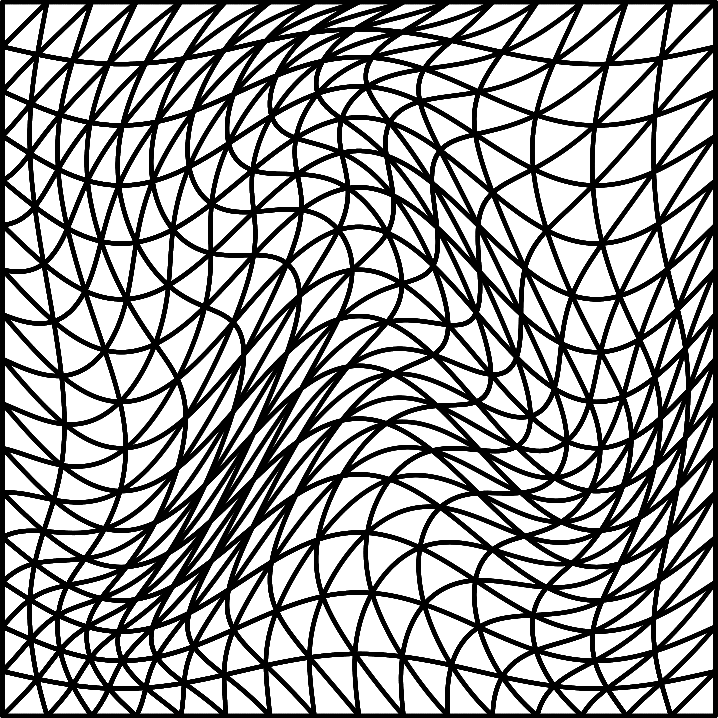
\includegraphics[width=.285\textwidth]{figs/wadgCurved.png}}
\subfloat[$f(\bm{x}) = e^{x+y}\sin\LRp{{\pi x}}\sin\LRp{{\pi y}}$]{
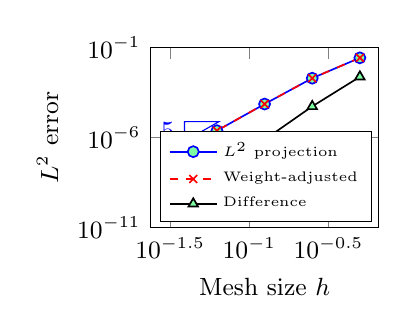
\begin{tikzpicture}
\begin{loglogaxis}[
    legend cell align=left,
    legend style={legend pos=south east, font=\tiny},
    width=.37\textwidth,    
    xlabel={Mesh size $h$},
    ylabel={$L^2$ error}, 
     ymin=1e-11, ymax=1e-1,    
    grid style=dashed,
] 

\addplot[color=blue,mark=*,semithick, mark options={solid,fill=markercolor}]
coordinates{(0.5,0.0268241)(0.25,0.00198388)(0.125,7.29929e-05)(0.0625,2.43094e-06)(0.03125,7.71592e-08)};
\logLogSlopeTriangleFlip{0.3}{0.15}{0.48}{5}{blue}
\addplot[color=red,mark=x,dashed,semithick, mark options={solid,fill=markercolor}]
coordinates{(0.5,0.0269391)(0.25,0.00197894)(0.125,7.29563e-05)(0.0625,2.43063e-06)(0.03125,7.71567e-08)};
\addplot[color=black,mark=triangle*,semithick, mark options={solid,fill=markercolor}]
coordinates{(0.5,0.00237193)(0.25,5.41179e-05)(0.125,7.6934e-07)(0.0625,1.18362e-08)(0.03125,1.84801e-10)};
\logLogSlopeTriangleFlip{0.3}{0.15}{0.225}{6}{black}

\legend{$L^2$ projection,Weight-adjusted,Difference}
%\legend{Uniform, Optimal, Smoothed}
\end{loglogaxis}
\end{tikzpicture}
}
\subfloat[$g(\bm{x}) = f(\bm{x}) + H(x+y-\sin(\pi x))$]{
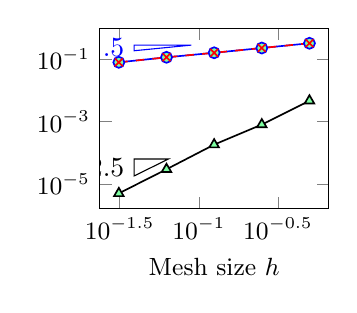
\begin{tikzpicture}
\begin{loglogaxis}[
    legend cell align=left,
    legend style={legend pos=south east, font=\tiny},
    width=.37\textwidth,
    xlabel={Mesh size $h$},
%     ymin=1e-7, ymax=1e1,
%    ylabel={$L^2$ error}, 
    grid style=dashed,
] 

\addplot[color=blue,mark=*,semithick, mark options={solid,fill=markercolor}]
coordinates{(0.5,0.323258)(0.25,0.227822)(0.125,0.160387)(0.0625,0.114753)(0.03125,0.0792918)};
\logLogSlopeTriangleFlip{0.4}{0.25}{0.875}{.5}{blue}
\addplot[color=red,mark=x,dashed,semithick, mark options={solid,fill=markercolor}]
coordinates{(0.5,0.324117)(0.25,0.227927)(0.125,0.160411)(0.0625,0.114756)(0.03125,0.0792924)};
\addplot[color=black,mark=triangle*,semithick, mark options={solid,fill=markercolor}]
coordinates{(0.5,0.00466574)(0.25,0.000804201)(0.125,0.000182886)(0.0625,2.96701e-05)(0.03125,5.01885e-06)};
\logLogSlopeTriangleFlip{0.3}{0.15}{0.18}{2.5}{black}

%\legend{$L^2$ projection,Weight-adjusted, Difference}
%\legend{Uniform, Optimal, Smoothed}
\end{loglogaxis}
\end{tikzpicture}
}
\caption{$L^2$ errors in approximating both smooth and discontinuous functions using $L^2$ and weight-adjusted projections on a curved mesh.  The approximation order is $N=4$, and a degree $2N$ quadrature rule is used to compute integrals over the reference triangle. }
\label{fig:superconverge}
\end{figure}

We next compare the approximation of the geometric factors on a curved three-dimensional mesh.  We generate a sequence of quasi-uniform unstructured meshes using GMSH \cite{geuzaine2009gmsh} and distort their coordinates using the mapping
\begin{align}
\bm{x} = \bm{x} + \frac{1}{8}\cos\LRp{\frac{\pi}{2}x}\cos\LRp{\frac{\pi}{2}y}\cos\LRp{\frac{\pi}{2}z}.  
\label{eq:mapping}
\end{align}
We then computed the maximum $L^2$ error in approximating $J^k\bm{G}^k_{ij}$
\[
\max_k \sqrt{\sum_{ij=1}^d \nor{J^k\bm{G}^k_{ij} - \tilde{J^k\bm{G}^k_{ij}}}^2_{L^2\LRp{\hat{D}}}}.  
\]

% alpha = 1/8
%coordinates{(0.737185,0.000791584)(0.39984,1.62016e-05)(0.166642,3.92283e-07)(0.0867136,5.76479e-09)};
%coordinates{(0.737185,0.00171192)(0.39984,8.52393e-05)(0.166642,2.31097e-06)(0.0867136,1.28404e-07)};


\subsection{Compressible Euler equations}

\subsubsection{Two dimensional experiments}

\note{Shock propagation on a curved mesh: testing entropy conservation}

\note{Isentropic vortex on curved and non-curved meshes}

\subsubsection{Three dimensional experiments}

\note{Isentropic vortex on curved and non-curved meshes}

\note{Taylor-Green vortex}

\section{Computational results}

The semi-discrete evolution equation is as follows
\[
\pd{\bm{u}}{t} = \LRs{\begin{array}{cc}
\bm{P}_q & \bm{L}_q
\end{array}}
\LRp{
\LRs{
\begin{array}{cc}
2\bm{D}_q & \bm{V}_q\bm{L}_q\\
\bm{V}_f\bm{P}_q & \bm{I}
\end{array} 
}\circ 
\LRs{
\begin{array}{cc}
\bm{f}_{S}(\bm{u},\bm{u}_f) & \bm{f}_{S}(\bm{u},\bm{u}_f)\\
 \bm{f}_{S}(\bm{u},\bm{u}_f) &  \bm{f}_S(\bm{u}_f^+,\bm{u}_f)
\end{array} 
}\bm{1}}.
\]
where $\bm{u}, \bm{u}_f$ are evaluations at volume and surface quadrature points.  

The method is outlined as follows: we store the conservation variables $\bm{u}$ at quadrature points, and compute projected entropy variables $\bm{v}_u = \Pi_N\LRp{\bm{v}(\bm{u})}$ 
\begin{enumerate}
\item Apply volume flux differencing ($\bm{D}_q$ and $\bm{V}_q\bm{L}_q$) and projection ($\bm{V}_q\bm{P}_q$) (volume kernel)
\item Apply surface flux differencing ($\bm{V}_f\bm{P}_q$) and lifting ($\bm{V}_q\bm{L}_q$) (volume kernel)
\item Apply WADG (scale by $1/J$ and apply $\bm{V}_q\bm{P}_q$ and update $\bm{u}$ at volume quad points.  Compute curvilinear projected entropy variables $\bm{v}_u = P_N^k \bm{v}(\bm{u}) =  \Pi_N\LRp{\frac{1}{J}\Pi_N\LRp{\bm{v}(\bm{u})J}}$, interpolate to volume quad points, and compute conservative variable volume values (update)
\item Interpolate entropy variables at surface quadrature points and write out conservative variable surface values (face).  
\end{enumerate}

\section{Conclusions}

\section{Acknowledgements}

The authors thank Mark H.\ Carpenter and David C.\ Del Rey Fernandez for informative discussions.

\bibliographystyle{unsrt}
\bibliography{dg}


\end{document}




%\section{Limiting}
%
%The evaluation of $\bm{u}_v = \bm{u}\LRp{\Pi_N v}$ can increase entropy pointwise, such that $S(\bm{u}_v) \geq S(\bm{u})$.  This can manifest as spikes in $\bm{u}_v$.  We wish to mollify the effect of such spikes.  
%
%The first approach is to limit the conservative variable $\bm{u}$
%\[
%\tilde{\bm{u}} = \bar{\bm{u}} + \Theta (\bm{u} - \bar{\bm{u}})
%\]
%where $\Theta$ is some diagonal matrix with entries in $[0,1]$.  We want to ensure that $\rho, E-\frac{\rho u^2}{2} > 0$.  
%
%The entropy for the compressible Euler equations is 
%\[
%U(\bm{u}) = -\frac{\rho s}{\gamma-1},
%\]
%where $s = \log\LRp{\frac{p}{\rho^\gamma}}$ is the physical specific entropy.  The entropy variables under this choice of entropy are then
%\begin{align*}
%v_1 = \frac{\gamma-s}{\gamma-1} - \frac{\rho u^2}{2p}, \qquad v_2 = \frac{\rho u}{\rho e}, \qquad v_3 = -\frac{\rho}{\rho e}.
%\end{align*}
%where the internal energy $\rho e = E - u^2/2$.
%
%The inverse mapping is given by 
%\[
%\rho = -(\rho e) v_3, \qquad m = (\rho e) v_2, \qquad E = (\rho e)\LRp{1 - \frac{v_2^2}{2 v_3}},
%\]
%where $\rho e$ and $s$ in terms of the entropy variables are 
%\[
%\rho e = \LRp{\frac{(\gamma-1)}{\LRp{-v_3}^{\gamma}}}^{1/(\gamma-1)}e^{\frac{-s}{\gamma-1}}, \qquad s = \gamma - v_1 + \frac{v_2^2}{2v_3}.
%\]
%The mapping is invertible so long as $\rho, E-\frac{\rho u^2}{2} > 0$, which can be ensured using standard limiters.  However, we have to ensure also that $\rho(\Pi_N\bm{v}) > 0$ (similarly for internal energy).  This boils down to ensuring that $\Pi_N v_3(x) < 0$, which guarantees that $(\rho e) > 0$ as well.   
%
%It can be helpful to ensure a stronger condition, that $\Pi_N v_3(x) \leq \max_{x} v_3(x)$.  This guarantees a bound constraint on the conservative variables evaluated using the projected entropy variables.  
%
%Another approach is to change the time-step size based on the difference between $\bm{u}$ and $\bm{u}_v$.  This would be similar to local time-stepping (high order interpolation of the numerical fluxes and multiple evaluations of )
%
%\begin{itemize}
%\item Adaptively choose time-step size?
%\item Expensive option: bisection or Newton algorithm for finding theta.  
%\end{itemize}


